%%
%% John Vandivier, GMU-formatted dissertation, "THREE ESSAYS ON THE ECONOMICS OF POSTSECONDARY ALTERNATIVE LEARNING"
%% Submitted to the GMU Library in May 2021 and defended June 1, 2021.
%% Derived from the GMU LaTeX PhD Dissertation Format Template
%%
%% Template Developed by:
%%      Daniel O. Awduche and Christopher A. St. Jean
%%      Communications and Networking Lab
%%      Dept. of Electrical and Computer Engineering
%%
%% Notes on usage can be found in the accompanying USAGE_NOTES.txt file.
%%
%%**********************************************************************
%% Legal Notice:
%% This code is offered as-is without any warranty either
%% expressed or implied; without even the implied warranty of
%% MERCHANTABILITY or FITNESS FOR A PARTICULAR PURPOSE!
%% User assumes all risk.
%% In no event shall any contributor to this code be liable for any damages
%% or losses, including, but not limited to, incidental, consequential, or
%% any other damages, resulting from the use or misuse of any information
%% contained here.
%%**********************************************************************
%%
%% $Id: GMU_dissertation_template.tex,v 1.7 2007/05/02 02:20:38 Owner Exp $
%%

\documentclass[11 pt]{report}
\usepackage{modifiedgmudissertation}
\usepackage{graphicx}
\usepackage{amsmath}                       %%
\usepackage{amsfonts}                      %%  for AMS mathematics
\usepackage{amssymb}                       %%
\usepackage{amsthm}                        %%
\usepackage[normalem]{ulem}                %   a nice standard underline package
\usepackage[noadjust,verbose,sort]{cite}   %   arranges reference citations neatly
\usepackage{setspace}                      %   for line spacing commands

\usepackage{booktabs}
\usepackage[hyphens]{url}
\usepackage{hyperref}
\usepackage{lineno}
\usepackage{longtable}
\usepackage{ragged2e}
\usepackage{siunitx}
\usepackage{tabularx}
\usepackage{threeparttable}
\usepackage{tikz}
\urlstyle{same}

\modulolinenumbers[5]
\graphicspath{{./figures-and-tables}}
\usetikzlibrary{calc,matrix}

% ref: https://tex.stackexchange.com/questions/50747/options-for-appearance-of-links-in-hyperref
\hypersetup{
    breaklinks = true,   %%% not grammatical
    hidelinks = true,    %%% not grammatical
}

\begin{document}

\onelinetitle{Three Essays on the Economics of Postsecondary Alternative Learning}
\author{John Vandivier}
\degree{Doctor of Philosophy}
\doctype{Dissertation}
\dept{Economics}

\seconddeg{Master of Public Policy}
\seconddegschool{George Mason University}
\seconddegyear{2015}

\firstdeg{Bachelor of Science}
\firstdegschool{University of Houston}
\firstdegyear{2012}

\degreeyear{2021}
\degreesemester{Summer Semester}

\advisor{Bryan D. Caplan}

\firstmember{First Member}
\secondmember{Second Member}
\thirdmember{Third Member}
\depthead{Department Head}
\deanITE{Dean's Name}

\titlepage
\copyrightpage
\dedicationpage

\noindent I dedicate this dissertation
to the satisfiable skeptic,
to the weirdo,
to the self-taught,
to the career switcher,
and to my children, current and future.

\bigskip

\noindent I encourage you to distinguish schooling from learning,
common wisdom from truth and falsehood,
a person from people,
and pain from evil.

\bigskip

\noindent Test all things; hold fast what is good.

% \noindent I encourage you to learn and act in balance as a single process,
% never confuse schooling for learning,
% celebrate friction and estrangement only if and always if it results from your pursuit of truth and love,
% and to test all things and hold fast to what is good.

\acknowledgementspage

\noindent I would like to express appreciation for four groups of people that have contributed to my doctoral education.
First, I would like to thank my dissertation committee.
Thanks to Dr. Caplan for reinvigorating the research on the return to university education.
The value of alternative education is interesting largely because it is comparable to such prerequisite work.
Thanks to Dr. Hanson for his contribution of big ideas into society and into my writing.
Thanks to the late Dr. Williams for his focus on improving the lives of individuals.
His focus was demonstrated with clarity of thought and speech inside and outside of the classroom.
Thanks to Dr. Klein for his kind and immediate commitment to join a dissertation-in-progress once Dr. Williams had passed away.

\bigskip

\noindent I would also like to thank Christina Vandivier,
a wonderful friend of mine from high school,
a fantastic mother,
and my wife.
I expect that I would not have attempted, much less obtained, doctoral education in her absence.

\bigskip

\noindent I would like to thank Mary Jackson for significant amelioration of the miscellaneous administrative inconveniences of graduate life.

\bigskip

\noindent Finally, I would like to thank my peers at George Mason University.
Many peers contributed to my success in and enjoyment of the program.
In particular, I would like to thank my regular study group.
The group included Rob Cripps, Bryan Cutsinger, Bob Hazel, Josh Ingber, Malhaz Jibladze, Slade Mendenhall,
Linan Peng, Patricia Saenz-Armstrong, and Garrett Wood.

%% // begin salty rant
% and also to my grandmother, many teachers, anon online individuals, and the media, for making me think a PhD is worth a damn
% and also to Jeff Bezos, Elon Musk, Mark Zuckerberg, Jack Dorsey, and others like them, who have provided me gainful employment prospects outside of academia and policy
%% // end salty rant

%%
%% Table of contents, list of tables, and lists of figures
%%

\tableofcontents
\listoftables
\listoffigures

%%
%% Abstract
%%

\abstractpage

This dissertation advances the field of education economics by describing the limits of competition between traditional and alternative postsecondary credentials in the United States. The results and conclusions contained in this set of three papers forms a substantive basis for change in policy, research, education provider behavior, and education consumer behavior. Evidence-based solutions that leverage these insights offer a solution to the student debt crisis, better social and private returns to education, education access improvements, and improvements to the quality and pace of learning.

The first essay,
\textit{Conformity and Soft Skills as Determinants of Alternatively Credentialed Non-College Graduate Hirability},
compares the skills gaps for college graduate and alternatively credentialed non-college graduate (ACNG) job applicants. I provide evidence that employers perceive a soft skills gap in ACNGs, and I demonstrate that employers see ACNGs as a labor pool with high quality variance, rather than a labor pool of general low quality. This paper provides a skill-level diagnostic that can be used by education providers to improve curricula.

%% Be sure to leave a line of whitespace immediately before this line!!!!!
%% (If this comment segment runs together with the preceeding text, you might
%%  see the second page of the abstract numbered "0".)
%%
%% If the abstract is more than one page, then place this line PRECISELY
%% at the page break; otherwise, comment it out.  (See note about this line
%% in the usage notes.)
%%
\abstractmultiplepage

The signaling model of education provides an ideal foundation for the questionnaire design that is utilized in all three essays. Where signaling model theorists have previously suggested that nonconformity creates a stigma for ACNG labor, I show that nonconformity is viewed as a net value add by employers. I propose that productivity variance risk aversion is a better explanation than stigma for the relatively weak average performance of alternative credentials to the traditional degree on the labor market.

The second essay,
\textit{Hirability and Educational Prestige},
tests the hypothesis that educational prestige explains hirability better than accreditation. Ordinary least squares and linear mixed model analyses provide evidence that prestige does explain a greater share of variance in hirability compared to accreditation, but the effect of accreditation also remains independently important. This paper identifies rules of thumb that education consumers can use to identify meaningfully high-prestige learning providers. These meaningful categories can also be used for further research into the return on investment in alternative education. Results suggest a need for accreditation reform to allow maximal social surplus in the market for education.

The third paper,
\textit{COVID-19 and Alternative Postsecondary Learning},
investigates the impact of the COVID-19 pandemic on social favorability to remote learning and alternative credentials. Results indicate that the pandemic increased favorability to remote learning and alternative credentials. The conclusion provides some reasons to think that high favorability will persist over time.

%%
%%  the main body of the dissertation
%%
\startofchapters


\chapter[Chapter 1: Conformity and Soft Skills as Determinants of Alternatively Credentialed Non-College Graduate Hirability]{}

\section{Introduction}

A substantial gap exists between the skills expected by employers and those possessed by college graduates\cite{mcgarry2016examination, malik2017great, abbasi2018analysis, gingras2000there}.
Experts view college alternatives,
including vocational school,
to be useful for technical training,
but the traditional college degree retains a wage premium over vocational education.
Unemployment, underemployment, and other adverse labor outcomes follow a similar pattern\cite{smith_2011}.
This paper seeks to resolve the apparent discrepancy between these outcomes while preserving the mainline economic view that employers pay for perceived job candidate skill.
% or expected marginal revenue product of labor
To explain the apparent discrepancy,
this paper tests the hypothesis that employers expect an offsetting non-technical skill deficit when considering an alternatively credentialed non-college graduate (ACNG).
I find evidence that employers and the general population in the United States expect a low level of soft skills from ACNG job candidates.

Alternative credentials refer to credentials other than the undergraduate degree\cite{brown2017complex}.
The category includes, for example,
industry certifications,
portfolios of work,
digital badges, and other records of unaccredited learning and achievement.
Consumers of alternative education typically intend to leverage alternative credentials toward better employment.
That is, they typically have the same goals as a college student.
Many individuals obtain alternative credentials as a supplement to a college degree.
Supplemental usage is excluded from the analysis in this paper.
This paper focuses on the use of alternative credentials as a substitute for a college degree.
% The level of analysis for this paper dives deeper than the level of credential into skill-level component signal analysis.
This paper provides a comparative analysis between traditional and alternative credentials at the skill level.
Education consumers and learning advisors can use results to inform strategic consumption.
Learning providers can use results as a skill-level diagnostic and product improvement resource.

% Alternative credentials can be obtained quickly and cheaply relative to college.
% Obtaining a college degree signals intelligence, conscientiousness, and conformity,
% but it may not signal technical skill\cite{horton_2020}.
% Alternative credentials signal technical skill.
% As such, they provide an effective supplement to a college degree.

% This paper is concerned with another use case in which a college degree is entirely substituted.
% In that situation, employers may apply a noncollege stigma.
% This is particularly the case for roles which are typically occupied by degree holders.
% Noncollege stigma is a presumption, expectation, or bias toward perception of a skill gap of a certain kind.
% Whether the gap exists in fact is out of the scope of the present paper.

% Technical skill generally implies intelligence.
% Alternative credentials, then, fail to signal two qualities compared to a college degree.
% Alternative credentials fail to signal conscientiousness and conformity.
% Interestingly, some employers may demand some level of nonconformity.
% Employers may also presume a certain lack of soft skill on the part of highly technical applicants.
% % Finally, employers may use alternative credentials as a proxy for other employee characteristics like income, education, race, and gender.

% % a missing link for future research: hirability only correlates with actual hiring decisions it isn't a hiring decision
% Hiring decisions reflect boundedly rational demand for skilled labor.
% a college degree and alternative credentials provide two qualitatively distinct signals of skilled labor.
% The hirability of individuals in possession of these credentials has been studied,
% but the underlying determinants are not clear.
% This paper hypothesizes that perceived skill gaps are important determinants of hirability.
% This paper further hypothesizes that perceived skill gaps are qualitatively different between college graduates and others.
% % In particular, this paper hypothesizes that a noncollege stigma is obtained for candidates without a degree in pursuit of roles typically filled by degree holders.
% % soft skill bias in particular

% three interesting follow-on questions:
%   1. do employers have such a bias
%   2. is such a soft skills gap presumption actually true
%   3. if true, due employers overvalue the soft skills gap
% related paradox: most people won't be in a job for 4-5 years,
% so why do they need to show conscientiousness and conformity towards the 4-5 year bachelor's goal line?
% hard skill stigma: in my experience, people who are highly technical are hard to work with
% soft skill bias: I am favorable bc i think u have soft skills (and maybe this is efficient...enter eq/iq discussion)

% This paper tests the hypothesis that there is a lack of hirability an ACNG (ACNG) is explained by an offsetting perceived lack in non-technical skills.
% In particular, this paper hypothesizes that ACNGs are seen as nonconformist and lacking in soft skills or non-technical skills.
% These deficits explain why an ACNG would not be a preferred source of labor in many cases,
% even if such a candidate does possess superior technical skill.

% technical skill has negative coefficient but magnitude and reliability (p-value/variance) are weaker; overall, less important effect
% hypothesis stems from signaling model.
% This paper proposes skill gaps are perceived in particular among soft skills for alternatively educated individuals.
% one might argue employers are mistaken here; technical work may involve higher, not lower, conscientiousness; ya maybe but out of scope.
% that is, we test social stigma and skill-level / decomposed stigma; an application of the signlaing model.

% Experts view college alternatives including vocational school as useful for technical training, but the traditional college degree retains a wage premium over vocational education.
% This paper hypothesizes that employers pay for skill.
% As a result, lower wages for technically skilled individuals are hypothesized to derive from an offsetting perception of skill deficit elsewhere.
% That is, this paper hypothesizes that employers view an ACNGs (ACNG) as lacking in soft skills.
% This paper hypothesizes that employers expect a skill deficit, although not a technical skill deficit, 
% This expected deficit explains the variance in labor outcomes.

% Sustained rising costs to higher education motivate periodic review of the return to a college degree.
% Despite rising costs, Americans have become more educated than expected over the past decade.
% Trades have contemporaneously seen a labor shortage.

% actually, trade school enrollment is increasing faster than undergraduate enrollment
% https://www.chronicle.com/newsletter/the-edge/2020-01-22
% By 2020, They Said, 2 Out of 3 Jobs Would Need More Than a High-School Diploma. Were They Right?
% overinvestment in college seems to cause a technical labor shortage, but the market is compensating by enrolling more technical folks too
% https://www.theatlantic.com/education/archive/2019/03/choosing-trade-school-over-college/584275/
% undergraduate enrollment has slowed recently and many employers have dropped a college degree requirement
% https://www.npr.org/2019/12/16/787909495/fewer-students-are-going-to-college-heres-why-that-matters
% it is not the case that employers are increasingly demanding a college degree, but it is the case that many do today. Let's examine their reasons.
% peak college?

% As of April 2021, Google Scholar results for the following search terms produce the following counts:
% "human capital theory": 72,300
% "signaling theory": 28,600
% "signalling theory": 16,600
% "screening theory": 4,540
% "control theory": 1,860,000
% "cultural capital theory": 3,830
% "institutional theory": 210,000
% "credentialist theory": 129
% "credentialism": 12,500
% 
% An undergraduate degree is a historically reputable investment.
In a noteworthy literature review, Bills identifies seven sociological or economic theories of the relationship between schooling and job assignment\cite{bills2003credentials}.
A keyword search in April 2021 indicates that human capital theory, institutional theory, and signaling theory are the three theories mentioned by Bills that are most frequently observed\footnote{
    A Google Scholar search for ``institutional theory'' yields about $210,000$ results.
    About two million results are found for control theory, but Bills notes that ``In its explanatory form, control theory is indistinguishable from human capital theory.''
    In addition, the keyword search results on control theory include disproportionately many results that do not relate to economic analysis.
    The search for `human capital theory' yields about $72,000$ results.
    The sum of `signaling theory' and `signalling theory' is about $45,000$ results.
    The total search result count for the other four theories is less than twenty-five thousand results.
    % The result counts are as follows:
    % "human capital theory": $72,300$,
    % "signaling theory": $28,600$,
    % "signalling theory": $16,600$,
    % "screening theory": $4,540$,
    % "control theory": $1,860,000$,
    % "cultural capital theory": $3,830$,
    % "institutional theory": $210,000$,
    % "credentialist theory": $129$
    % "credentialism": $12,500$,
}.
% The application of institutional theory to education involves `holding constant what they may have learned in school'.
When applied to the economics of education, the institutional theory holds that an institution improves individual labor prospects by declaring some individuals to be graduates.
In this application, institutional theory can be included in a signaling model with institutional effects.
In the current study, institutional effects are held constant by using hypothetical questions involving anonymous institutions.
% line above is sus bc we don't name institutions but we distinguish college grads from ACNGs,
%     and accreditation per se may have some effect that is arguably institutional in a sense
%     but, my conclusions are fine bc i interpret the signal and allow and even suspect that actual skills deviat from signalled skills for grads and acngs

% The signaling model is one of the two standard explanations of the relationship between credentials and labor outcomes\cite{weiss1995human}.
For the purpose of this study, signaling theory provides three advantages over the alternative human capital theory.
First, signaling theory can explain labor outcome variance when human capital unobserved\cite{weiss1995human}.
By extension, signaling theory can also explain labor outcome variance when human capital is held constant.
% First, signaling theory is able to explain labor outcome variance across labor types when skills are totally equal.
% Under a human capital model, in contrast, a variety of labor outcomes would directly imply variance among input labor.
% The present paper expects that skills for the ACNG compared to other labor types are not totally equal, but this must emerge as a result rather than a presumption.

Second, the signaling model empowers a questionnaire research design.
In a standard human capital model of wages, human capital is an input to a production function\cite{hellerstein2007production}.
In a competitive labor market, firms are willing to pay wages equal to the marginal revenue product.
% often MRP is flatly called productivity and defined as human capital
The marginal revenue product for an individual is a function of human capital factors, including skills.
Establishing a wide array of such skill measures would be complicated and prone to measurement sensitivities, assumptions, and errors of various kinds.
In this framework, a questionnaire is a second-best design that provides a proxy for the functional measure of skill.

Signaling theory takes the reverse approach.
According to the signaling model, willingness to pay is a function of perceived quality.
The relationship between perceived quality and actual quality is secondary.
In this framework, a questionnaire is an ideal measurement tool.
The value of this research approach is supported by the broad use of questionnaires
to identify willingness to pay within the field of market research\cite{ingenbleek2013best}.

% In this framework, a questionnaire is a direct measure of the functional construct, which is the opinion of the employer.
An additional benefit of using a questionnaire is the ability to ask hypothetical questions.
Hypothetical questions avoid the problem of unobserved heterogeneity
because the analyst has total knowledge over the subject of measurement.

Third, signaling theorists have laid out a testable hypothesis for weak labor outcomes among non-college graduates.
Following this model, scholars claim that the college degree signals intelligence, conscientiousness, and conformity\cite{caplan2018case}.
This paper hypothesizes that, in contrast, alternative credentials signal nonconformity and low conscientiousness.

% Proponents of the signaling model often prefer employer-oriented explanations of college enrollment.
% In this explanation, employers prefer college graduates because the college degree signals intelligence, conscientiousness, and conformity.
% While a technical credential signals intelligence and technical skill, the absence of a degree yields a perceived gap in the mind of the employer.
% There is a perceived comparative lack on the part of the non-college graduate with respect to conscientiousness and conformity.
% This paper tests this hypothesis.

% An agent-based explanation would be that high school graduates are not taught about these alternatives.
% The college degree is popular, has a well-defined return, and is low in risk.
% Particular alternative programs are obscure and often lack a well-defined return.

% Other research indicates that conscientiousness and conformity are not always desirable labor qualities.
% There is some reason to doubt the hypothesis that lower perceived value is attributable to signaling differences in conscientiousness and conformity.
% Research indicates that extreme values for either factor in either direction may be detrimental to productivity.

% TODO: long paper food...uncomment below section as it implies we should be doing marginal analysis. Then do marginal analysis, and K*K skill interactions
% TODO: maybe move to results section when we talk about conscientiousness
% Research indicates a goldilocks level or bliss point for both conscientiousness and conformity is likely to exist.
Employer demand for conscientiousness and conformity follows a bliss point pattern.
Excess individual conscientiousness can disturb team performance\cite{curcseu2019personality}.
Conformity can lead to a lack of innovation and suboptimal organizational practices\cite{symon2006neglected}.
% Psychologists also state that
Conformity selection occurs in part through heuristic cognition or unconscious bias.

% Because a single measure operationalizes each of these effects and their own negation, a fixed sample size is relatively unlikely to identify an important coefficient.
% Because these factors are sometimes demanded and in other cases the inverse is demanded, a factor coefficient may be harder to identify and may only represent the average effect, even if the average effect is hardly predominant in practice.

% The psychological problem is related to but distinct from the pure logical problem that a totally conformed mind is necessarily incapable of innovation.
% Firm innovation requires an underlying capacity for individual innovation.
% Firms must have some capacity for innovation to sustain profit in a growing economy.
% Even if conformity selection is a correct explanation of ACNG aversion, then, it may not be an ideal practice when viewed through the lense of technical or economic efficiency.
% Risk aversion is compatible with a sometimes-concious, sometimes-heuristic decisioning model.

% Innovators, leaders, and high-performers are three kinds of virtuously nonconformant labor.
% Because conformity is sometimes undesirable and sometimes desirable,
% the effect may neutralize itself in an ordinary OLS stastistical analysis.
% The effect may not be identified as important or significant in any particular direction.

Risk aversion is a distinct explanation for conformity selection.
Some employers are not able to evaluate an alternative credential with confidence.
Such an employer views ACNG labor as a gamble with some odds of positive or negative outlier value.
The employer may not prefer to hire such a candidate due to risk aversion,
even if their point estimate for ACNG labor value is higher than their point estimate for a recent college graduate.
If firm size effects are positively associated with ACNG hirability, this will add weight to an explanation based on risk aversion.
% Reasons for this include: 1) failure to deliver can be catastrophic, so low performers may be disproportionately untolerable.
% Revenue consistency, timeline, reputation, quantity produced targeting, large min skill labor cost and marginally small pay increase to achieve adequate production.
% Performance monitoring and turnover costs reinforce this
% zb states I'm assuming constant cost per hire...actually I allow that some portion of large-firm hirability is due to better ability to distinguish low vs high
% other than that effect, the remainder would be attributable to risk aversion.
% yes, the null hypothesis is no difference in cost per hire; but I can also support that which I suspect...turnover costs are proportionally smaller for large firms
% these firms are able to specialize and economize in hiring, plus they are more likely to have high-skill candidates that can better interview and recruitment tech+processes that scales
% TODO: long paper food... consider below articles and flesh out the risk aversion to firm size interaction thing
% note turnover cost calculation is complex but we proxy of just cost to hire. A + B below support cheaper for large firms. (C reinforces B)
%   A) "As stated in a study by the National Association of Colleges and Employers, hiring an employee in a company with 0-500 people costs an average of $7,645."
%   B) "Another study by the Society for Human Resource Management states that the average cost to hire an employee is $4,129, with around 42 days to fill a position."
%   C) "According to Glassdoor, the average company in the United States spends about $4,000 to hire a new employee, taking up to 52 days to fill a position."
% related but doesn't solve the issue: https://builtin.com/recruiting/cost-of-turnover
% https://toggl.com/blog/cost-of-hiring-an-employee
% The highest performing employers, however, will be able to distinguish desirable from undesirable candidates within the unconventional pool.
% Risk aversion varies naturally among firms. <- probably don't write this line in paper as a reviewer can always posit there is a further reason you are missing
% Some employers that are high in risk aversion will provide a net preference to ACNG due to nonconformity preference.

% TODO: long paper food...below section is part of intro or perhaps model...
% \subsection{Process Explanations of Suboptimal Wages}

% Basic price theory holds that an employer should pay wages equal to the marginal revenue product of labor.
% In the real world, measuring candidate productivity at hiring time is costly and imperfect.
% % This produces a technical error which assumes alignment between the goals of the firm and a hiring team.
% A further issue is identified when the hiring team is scrutinized for principal-agent problems.
% The hiring team is composed of individuals with preferences, calculative limitations, and other biases.
% Monitoring and correcting for these problems is expensive,
% so firms will heterogenously realize some aggregation of these individual definiciencies.

% Exacerbating the already necessarily imperfect hiring process are candidate-side problems.
% Firms must hire among a finite, potentially small, number of candidates.
% Risk aversion to time expense and other search costs may lead a firm to approve a suboptimal candidate\cite{simon1976substantive}.
% In some cases, candidate pools may be systematically problematic.
% In law and medicine, for example, extensive education and training are legally required.
% These policies further restrict the candidate pool, inflate expected wages, and systematically alter the content of education in a politically-motivated manner.
% Market forces implement hiring as a lumpy expenditure process to begin with, but certification requirements, wage regulation, and other policies extend the problem.

% The prior discussion highlights many locations of hiring process inefficiency.
% The practical importance of magnitudes and kinds of such effects are described in a legion of related papers.
% A meager sampling of five such effects would include the attractiveness effect and many other issues related to gender bias\cite{quereshi1986physical},
% agentic behavioral stigma\cite{steffens2009feminization},
% and complex biases related to communication style\cite{brouer2017gender, nijs2019effects, sampugnaro1983nonverbal}.
% Sung et al find that impression management meaningfully weakens disability stigma\cite{sung2017disclose}.
% These tactics are transferable in part to noncollege stigma mitigation.
% Finally, there are a wealth of concerns about the effects of social media.
% For one, it presents a channel for the revival of religious discrimination\cite{esposito2018signaling}.

% In the face of so many important inefficiencies, one begins to wonder whether the original theory holds any water at all.
% Papers which identify matching effects, including the present paper,
% serve to limit the proportion of explanation attributable to bias and redeem the elementary price theory story to some extent.
% Prior work demonstrates the important of matching effects in the form of norm compliance\cite{francesco1981gender}.
% Meta-accuracy is a kind of matching measure, and it has been shown to move positively with hirability\cite{renier2018no}.

% \section{Literature Review}
% TODO: long paper food...lit review exists in Announcement effects in the cryptocurrency market
% TODO: long paper food...expand on the signaling model vs the human capital model
% Faster and cheaper alternatives to college exist, but high schools prefer immediate college enrollment over alternative options at a rate of nearly 2:1.
% A New U: Faster + Cheaper Alternatives to College
% Faster and cheaper alternatives to college exist, but the typical student prefers to immediately enroll in college.
% Five student-oriented explanations include an inflated perception of the return to college,
% lack of awareness about alternative programs,
% social pressure to pursue college over alternatives,
% inability to confidently compare returns to alternatives,
% and risk aversion which favors college as a low-risk option despite high cost.


\section{Data and Methodology}
% my model is similar to a Mincer earnings function...but it's not earnings (i could switch income around and maybe get a kind of that)
% https://en.wikipedia.org/w/index.php?title=Mincer_earnings_function&oldid=994739612

A simple model of demand for labor provides context for the hypothesis of interest.
This model is clarified in Equations \ref{eq1} and \ref{eq2}:

\begin{subequations}
    \begin{equation}
        % maybe S is not S_j showing S is a non-person-specific credential
        % but I like S_j because it is *those credentials possessed by j* which can be a unique collection + unique work history, other unique signal, etc...
        S_j = f(H_j)
        \label{eq1}
    \end{equation}
    \begin{equation}
        w_{ij} = E_i(MRP_j) = f_i(S_j)
        % alternatively, D_i(L_j) = E_i(MRP_j) = f(S_j, i)
        \label{eq2}
    \end{equation}
\end{subequations}

Job candidate $j$ generates a signal of productivity $S_j$ from unobserved human capital $H_j$.
Employer $i$, forms an expectation of the marginal revenue product of $j$ on the basis of $f_i(S_j)$, an employer-specific evaluation of $S_j$.
A specific employer is willing to pay a specific job candidate wages of $w_{ij}$.

This study uses ordinary least squares (OLS) regression analysis to estimate the effect of perceived skill gaps on hirability.
An employer is willing to pay more for a relatively hirable individual.
The representation of willingness to pay makes hirability a proxy of demand for labor and $w_{ij}$.
% measure or proxy? proxy bc diff units.
% this is questionable because hirability is technically the willingness to execute a wage integrated over some expected time period (average employee tenure)
% but then, that integrated wage would just be wage multiplied by some constant and we would need to divide by some constant since hirability is a probability
% so, hirability should correlate directly to wage after all
% you also might say hirability is theoretically closer to an estimate of productivity...but who cares it's once again equal
% and we want to frame the overall model as a simple labor demand model.
%
% Equally, a respondent is making an expected productivity statement when scoring hirability
% This study presumes that employers are willing to pay less for an ACNG.
% This study also presumes that ACNG labor has better technical skill.
This paper hypothesizes that employers preferentially value soft skills in the course of $f_i(S_j)$
to explain the reduced willingness to pay for ACNG labor relative to college graduate labor.
If employers do bias toward soft skills in job candidate evaluation,
one or more soft skill gap factors should yield a negative coefficient
in a regression on hirability.

This paper leverages an original set of online questionnaire responses ($n = 322$).
Responses are cross-sectional data obtained in early February of 2021.
Respondents are United States citizens at or over the age of eighteen.
Qualified respondents participated in the survey through the Amazon Mechanical Turk platform.

The survey includes 65 questions in two sections\footnote{See Appendix A for a full copy of the survey.}.
The first section captures respondent characteristics, and the second section captures a skill-level evaluation of various hypothetical job candidates.
Grouping these variables into three groups simplifies discussion.
There is the dependent variable of interest, independent variables of interest, and categorical controls.

In this study, the categorical variables and the control variables are the same set.
The independent and dependent variables of interest are Likert-type responses on a 10-point scale
% Employer responses did not significantly differ from the general population,
% so results generally hold for both employers and the United States population.
\footnote{
    It is an accepted practice to treat Likert-type responses as either categorical or continuous for regression analysis.
    % This paper treats such variables as continuous, which is consistent with the theoretical structure of the demand curve and the other variables of analysis.
    % it's also consistent with normalized reporting of real skill measurement; even percentiles themselves are continuous entities.
    % ie, I could do marginal analysis; and i did a little but i'm not talking about it lol.
    Jaccard and Wan provide support for continuous analysis of Likert-type data.
    They note that severe departures from the assumptions on cardinality ``do not seem to affect Type I and Type II errors dramatically,''
    particularly when the Likert scale is five or more points\cite{jaccard1996lisrel}.
    This paper uses a 10-point scale and treats these data as continuous.
    % A 10-point scale is equivalent to a continuous response from 1 to 10 with rounding.
    %
    % In the current data set, continuous treatment provides a consistent and conservative fit of the data with high confidence.
    % Categorical decomposition yields higher fit with less significance in each category of Likert response.
    % This indicates categorical decomposition may represent a case of overfit and is therefore an additional reason not to prefer that analytical approach.
    %
    % % TODO: long paper food...add marginal fx and u get a third reason Likert as continuous is gtg
    % Finally, treating Likert-type responses as continuous is structurally defensible in this particular study.
    % The notion that Likert-type responses are purely ordinal would make the notion of marginal effect absurd and incalculable,
    % but willingness to pay for labor, conscientiousness, and other factors used in this study are known to exhibit marginal effects in the literature. % TODO: I could cite but it's pretty obv
    % See the results section where a marginal effect from conscientiousness is identified and interpreted in a meaningful way.
    %
    % TODO: but probably not...I could also cite a paper where an economist uses Likert questionnaire data as cardinal
    % i would be happy to use a categorical-like treatment if not for this, and the latter might even have better fit but it could be overfit.
    % finally, an alternative approach would be to treat likert responses as categorical, but the continuous treatment has less fit and more structural justification
    % categorical treatment is a relative overfit
    % likert-type units can be considered direct psychological measures or economic proxies.
    % The likert-type response curve can be thought of as a function of actual skill;
    % b. decent paper on ordinal independent variables: https://www3.nd.edu/~rwilliam/stats3/OrdinalIndependent.pdf
    % c. more on this: https://www.researchgate.net/post/Is_a_Likert-type_scale_ordinal_or_interval_data
}.
Higher Likert-type values indicate greater agreement with the associated statement.
Categorical controls include state of residence,
the industry of occupation,
employer status,
firm size,
and a measure called duration.

% https://stats.stackexchange.com/questions/539/does-it-ever-make-sense-to-treat-categorical-data-as-continuous
% I treat duration as continuous even though it is categorical, but the likert-type defense applies statistically.
Duration measures the length of time the respondent believes it takes to obtain an alternative credential.
Employer status describes whether an individual makes hiring and firing decisions in the course of their employment.
The variable takes one of three values: yes, no, or unemployed.
Employer effects refer to the case where an individual states that they do make hiring and firing decisions.
State of residence refers to a state within the United States or the District of Columbia.
% While it was permitted, only one actual response identified the District of Columbia as a residence.

The dependent variable of interest is called hirability.
Hirability measures agreement that, ``For many professions, alternative credentials can qualify a person for an entry-level position.''
The dependent variables of interest include perceived skill gaps and rulebreaker effects.

% The unit of factor coefficients for nonconformists and skill gaps is hirability per Likert-type unit, where hirability is also a Likert-type unit.
% Rulebreaker effects refer to a collection of three factors that describe the way employers think about nonconformists, or "People who are willing to break formal or informal rules and norms."
Rulebreaker effects refer to a collection of three factors that measure respondent agreement with statements about nonconformists, or ``People who are willing to break formal or informal rules and norms.''
% The three rulebreaker questions measure respondent agreement with statements 
The first statement indicates that nonconformists present a risk to a company's reputation, productivity, or value.
This statement received the least agreement and greatest response variance
among three qualitatively different descriptions of nonconformists ($\mu = 6.29, \sigma = 2.51$).

The second statement indicates that nonconformists are held back by rules,
and ``could just as easily be high performers as low performers.''
% The second statement indicates that people break rules which hold them back, and that nonconformists "could just as easily be high performers as low performers."
% MAYBE TODO: standard error instead of or in addition to standard deviation. maybe make a table since there are at least three cases of similar report.
This statement received the most agreement and least variance among rulebreaker statements ($\mu = 6.93, \sigma = 2.10$).
The agreement with this statement provides evidence against the thesis that employers value conformity for its own sake.
In turn, this adds weight to the theory that employers value conformity as a risk aversion tactic while knowing that nonconformity signals positive outlier potential.
The third rulebreaker effect states that rulebreakers are creative, innovative, and likely to benefit company culture ($\mu = 6.71, \sigma = 2.18$).
% managers are wary of ACNG, having high correlation with "Rule Breakers Risky"
% reg _ismanager1 rulebreakersnormsmightbedoingsob rulebreakersnormsprobablyhaveaha rulebreakersnormstendtobegiftedi

% % MAYBE TODO: sentence below can be shortened and we can introduce likert-type unit as distinct from likert-type response since it's a computed value
% Perceived skill gaps are computed from perceived skill questions in the second section of the survey.
% % Respondents do not directly report perceived skill gaps.
% % Instead, responses indicate perceived skill level for particular skill and a particular type of job candidate.
% % 13 skills are analyzed and 4 job candidate types are surveyed, for a total of 52 questions in the second section on perceived skill.
% % MAYBE TODO: citation to "make response anchoring appropriate"
% % Each section begins with a contextual message to normalize response anchoring.
% % Questions are provided in nonrandom order for the same reason.
% % Data from the second section is used to calculate perceived skill gaps.
% For each of 13 skills, the respondent is asked to imagine four types of job candidate.
% One type of candidate is an ideal candidate.
% Raw perceived ACNG skill gaps are calculated by differencing the perceived skill of an ideal candidate with the perceived skill of an ACNG.
% % technically, the actual skill of an ideal candidate equals the perceived skill so the adjective is extraneous; but let's be consistent and not confuse reader.

Rulebreaker effects and perceived skill gaps are structurally linked.
One of the skills that respondents evaluate is nonconformity, or ``willingness to break formal or informal rules and norms.''
Interpreting rulebreaker effects jointly with the conformity gap effect
% Joint interpretation of nonconformity and rulebreaker effects
enables better explanatory power and diagnostic utility.
% Explanatory power is improved because conformity has potential benefits and costs.
% Aggregating these effects under a single variable creates noise.
% Explanatory power is improved because employers can express that they value conformity either per se or as a proxy for some other qualities.
% Diagnostic utility is improved because alternative learning providers may be able to accomodate whatever non-per-se qualities employers value.

Perceived skill questions in the second section of the survey allow for two ways to calculate perceived skill gaps.
Perceived skill gaps are measured separately with and without overqualification effects.
Overqualification effects are important in external research\cite{green2007there, raybould2005over}, but skill gap analysis that ignores these effects is also routine\cite{blake_2018}.
% MAYBE TODO: cite more than 1 person who ignores overqualification
% MAYBE TODO: just have one dependent variable and don't mention the other. it's something i did at analysis time, but may be confusing in the paper.
%       alternatively, keep 'em both and call the second a robustness test...that is what i use it for anyway

Perceived skill is a Likert-type response reporting agreement stating that a particular candidate has a particular skill.
For each of 13 skills, the respondent imagines and reports skill levels for the ideal candidate,
the average actual employee,
the average recent college graduate,
and the average ACNG.
As a result, 52 of the 65 questions in the survey are questions on perceived skill about kind of candidate.

The raw skill gap for a candidate is the difference between the perceived skill for that candidate and the ideal candidate.
The perceived skill gap with overqualification effects equals the raw perceived skill gap.
The perceived skill gap without overqualification is zero if the raw skill gap is negative,
and otherwise, it is equal to the raw skill gap.

The concept of skill is intentionally treated loosely in this analysis.
The thirteen factors treated as skills include
attractiveness,
verbal, written, and body language communication skills,
conscientiousness,
customer service skill,
emotional intelligence (EQ),
expected salary,
teamwork,
technical skill,
willingness to break formal or informal rules (nonconformity),
willingness to work odd hours,
and willingness to commute.
% TODO: discuss attractiveness halo effect

Results focus on ACNG skill gap coefficients
and also comparative skill gaps between ACNG labor and recent college graduates.
Perceived ACNG skill gaps are also called absolute skill gaps.
Subtracting the perceived recent college graduate skill gap from the absolute skill gap yields the comparative skill gap.
% In this study, overqualification effects ended up reducing explanatory power, so they are largely ignored.

Models of these variables will support the hypothesis if soft skills are more important than technical skill gaps.
Significant rulebreaker effects would provide evidence that conformity is valued differently for different types of employers.
A positive relationship between firm size and hirability would support an explanation from risk aversion.
% MAYBE TODO: I also expect signs to be generally negative and soft skills should be statistically significantly less for ACNG compared to recent college graduate

% simple match effect: those that prefer technical talent will tend to support alternative credentials.
% complex match effect: a match profile will have significantly and importantly more explanatory power compared to but consistent with a simple match effect.

% quality question meta: 1 to 10: disagree to agree
% ---
% An ideal candidate would have this quality...
% A typical employee would have this quality...
% A college graduate would have this quality...
% A credentialed or certified non-college graduate would have this quality...
% [later] Someone who is self-taught (without a credential or portfolio) would have this quality...
% [later] A typical junior-level high school student would have this quality...

% some notes, mainly out of scope
% ---
% hiring error awareness increases in a few ways
%  1. [passive search] participant observation. As an interviewer, interviewee, hiring manager, or other professional involved in the process, I simply notice a problem
%  2. [passive search] passive company and individual level search into HR best practices; an industry newsletter says hey Griggs v Duke happened so don't use IQ tests anymore.
%  3. [passive search]: audit compliance (legal+required, or optional audits from firms that certify quality, for example)
%       example: Supreme Court case Griggs v Duke had an industry-wide effect thru this means
%  4. [active search] intrapraneurship / policy change championing begins with an individual saying hey let's investigate this thing. what would motivate such individual? (maybe due to 1 or 2).
%
% my prior work has shown that we can predict (r2 0.5 - 0.7 and ar2 0.3 - 0.6) alternative education hirability from employer factors alone - without concern to matching

\section{Results}

% Hirability in this study is called favorability in the COVID study.
% Here, I want to highlight the theoretical connection to willingness to pay.
% In the other study, I wanted to highlight the psychometric connection to familiarity bias and so forth
The median hirability response was eight out of ten.
The mean response is about 7.42.
% Of 322 responses, 10 responses indicate a hirability of less than four out of ten.
% Partial responses were submitted in 21 cases, but partial responses did not impact factors in models of interest.
Absolute skill gaps and comparative skills gaps are both important explanations of hirability.
Soft skills explain hirability better than technical skill does in both absolute and comparative terms.
Technical skill is not a contributing factor in any model of interest.
Of the thirteen skills investigated, seven skills contribute to the preferred model.

% TODO: skill gap ols, gap of gaps ols

% TODO: final ols

% TODO: consider RLM, GLM, and control variables.

% TODO: maybe Compare directly to bootcamp results from Indeed: https://www.indeed.com/lead/what-employers-think-about-coding-bootcamp

% TODO: in preferred model, discuss Duration forced in, don't worry bout multicollinearity bc N/A dropped; rulebreaker gaps forced in

% \subsection{A Model of Absolute Skill Gaps}

Table \ref{tab:table_new_ols} reports five interesting multiple regressions.
Models 1 through 4 maximize adjusted r-squared for a given set of factors.
Factors in these models are not constrained using a p-value threshold.
Model 4 is the preferred model, and factors in this model have a p-value less than $0.28$.
Model 5 is a special case designed to answer an analytical question.

Models 1 and 2 maximizes adjusted r-squared using absolute skill gaps.
Model 1 includes overqualification effects, and Model 2 excludes these effects.
This model is useful to demonstrate which skills are important determinants of ACNG hirability.
The key result from these two models is that measuring skill gaps without overqualification is preferred.

Models 3 through 5 also exclude overqualification effects.
Model 3 maximizes adjusted r-squared using comparative skill gaps.
This model explains hirability by comparing ACNG labor to recent college graduates by skill.
Model 4 synthesizes comparative and absolute skill gaps.

% derived from analysis-5-regs-table.do
{
\def\sym#1{\ifmmode^{#1}\else\(^{#1}\)\fi}
\begin{tabular}{l*{5}{c}}
\toprule
                         &\multicolumn{1}{c}{1}&\multicolumn{1}{c}{2}&\multicolumn{1}{c}{3}&\multicolumn{1}{c}{4}&\multicolumn{1}{c}{Model 5}\\
\midrule
Is Employed Non-Manager  &      -0.336         &      -0.383\sym{*}  &      -0.497\sym{**} &      -0.471\sym{**} &      -0.451\sym{**} \\
\addlinespace
Is STEM Worker           &      -0.491\sym{**} &      -0.529\sym{**} &      -0.525\sym{**} &      -0.557\sym{**} &      -0.564\sym{**} \\
\addlinespace
Employees 51-200         &      -0.475\sym{*}  &      -0.480\sym{**} &      -0.364         &      -0.459\sym{*}  &      -0.457\sym{*}  \\
\addlinespace
Industry Credentials Legally Required&       0.706\sym{*}  &       0.722\sym{**} &       0.374         &       0.378         &       0.375         \\
\addlinespace
Industry Credentials Normal&       0.932\sym{**} &       0.926\sym{**} &       0.487\sym{*}  &       0.436\sym{*}  &       0.448\sym{*}  \\
\addlinespace
Industry Credentials Sometimes Used&       0.467         &       0.475         &                     &                     &                     \\
\addlinespace
Industry Credentials Unknown&       0.641\sym{*}  &       0.684\sym{**} &                     &                     &                     \\
\addlinespace
Industry, Agriculture    &       1.368         &       1.619\sym{*}  &                     &                     &                     \\
\addlinespace
Industry, Energy         &      -1.277\sym{*}  &      -1.190\sym{*}  &      -1.200\sym{*}  &      -1.442\sym{**} &      -1.448\sym{**} \\
\addlinespace
Industry, Finance, Investment, or Accounting&      -0.811\sym{***}&      -0.783\sym{***}&      -0.712\sym{***}&      -0.715\sym{***}&      -0.717\sym{***}\\
\addlinespace
Industry, Information Technology&       0.335         &       0.264         &       0.438\sym{*}  &       0.306         &       0.337         \\
\addlinespace
Industry, Law            &      -1.813\sym{***}&      -1.670\sym{**} &      -1.935\sym{***}&      -1.876\sym{***}&      -1.857\sym{***}\\
\addlinespace
Industry, Transportation &       1.512\sym{*}  &       1.643\sym{**} &       1.216         &       1.403\sym{*}  &       1.350\sym{*}  \\
\addlinespace
State, Arizona           &      -1.157\sym{**} &      -1.048\sym{**} &      -0.755         &      -0.823\sym{*}  &      -0.790         \\
\addlinespace
State, Arkansas          &      -2.690\sym{***}&      -2.817\sym{***}&      -2.489\sym{***}&      -2.664\sym{***}&      -2.770\sym{***}\\
\addlinespace
State, California        &      -0.575\sym{*}  &      -0.570\sym{**} &      -0.488\sym{*}  &      -0.435         &      -0.446         \\
\addlinespace
State, Colorado          &      -1.446\sym{**} &      -1.423\sym{**} &      -1.463\sym{**} &      -1.521\sym{***}&      -1.508\sym{***}\\
\addlinespace
State, Connecticut       &      -1.401         &      -1.550         &                     &                     &                     \\
\addlinespace
State, Florida           &      -0.444         &      -0.454         &                     &                     &                     \\
\addlinespace
State, Hawaii            &      -3.232\sym{***}&      -3.271\sym{***}&      -2.884\sym{***}&      -2.869\sym{***}&      -2.812\sym{***}\\
\addlinespace
State, Illinois          &      -0.637         &      -0.699\sym{*}  &      -0.596         &      -0.675\sym{*}  &      -0.698\sym{*}  \\
\addlinespace
State, Kansas            &      -3.283\sym{**} &      -3.486\sym{**} &      -2.923\sym{*}  &      -3.116\sym{**} &      -3.101\sym{*}  \\
\addlinespace
State, Kentucky          &      -3.143\sym{***}&      -3.167\sym{***}&      -2.583\sym{***}&      -2.729\sym{***}&      -2.679\sym{***}\\
\addlinespace
State, Louisiana         &      -1.455\sym{*}  &      -1.255\sym{*}  &      -0.915         &      -0.941         &      -0.898         \\
\addlinespace
State, Maryland          &      -0.596         &      -0.642         &                     &                     &                     \\
\addlinespace
State, Nebraska          &      -2.037\sym{*}  &      -2.167\sym{*}  &      -1.391         &      -1.655         &      -1.596         \\
\addlinespace
State, Nevada            &      -1.406         &      -1.470         &      -1.465         &      -1.434         &      -1.409         \\
\addlinespace
State, New Jersey        &      -1.145         &      -1.139         &      -0.976         &      -0.936         &      -0.963         \\
\addlinespace
State, New York          &      -0.692\sym{**} &      -0.640\sym{*}  &      -0.617\sym{*}  &      -0.595\sym{*}  &      -0.590\sym{*}  \\
\addlinespace
State, Ohio              &      -3.943\sym{***}&      -4.024\sym{***}&      -4.051\sym{***}&      -3.808\sym{***}&      -3.761\sym{***}\\
\addlinespace
State, Pennsylvania      &      -0.752         &      -0.687         &      -0.608         &      -0.534         &      -0.539         \\
\addlinespace
State, South Carolina    &      -1.183         &      -1.243         &      -1.361         &      -1.310         &      -1.347         \\
\addlinespace
State, Tennessee         &      -1.878\sym{**} &      -1.909\sym{**} &      -1.545\sym{*}  &      -1.843\sym{**} &      -1.799\sym{**} \\
\addlinespace
State, Texas             &      -0.906\sym{**} &      -0.851\sym{**} &      -0.797\sym{**} &      -0.790\sym{**} &      -0.789\sym{**} \\
\addlinespace
State, Washington        &      -0.817         &      -0.863\sym{*}  &      -0.880\sym{*}  &      -0.996\sym{**} &      -1.003\sym{**} \\
\addlinespace
Duration                 &       0.666\sym{**} &       0.634\sym{**} &       0.811\sym{***}&       0.744\sym{**} &       0.719\sym{**} \\
\addlinespace
cduration2               &     -0.0884\sym{**} &     -0.0857\sym{**} &      -0.113\sym{***}&      -0.103\sym{**} &     -0.1000\sym{**} \\
\addlinespace
WOQ, Gap, Attractiveness &      -0.161\sym{***}&                     &                     &                     &                     \\
\addlinespace
WOQ, Gap, Body Language-IT&       0.100         &                     &                     &                     &                     \\
\addlinespace
WOQ, Gap, Conscientiousness&     -0.0657         &                     &                     &                     &                     \\
\addlinespace
WOQ, Gap, EQ             &     -0.0966         &                     &                     &                     &                     \\
\addlinespace
Rule Breakers Risky      &      0.0732\sym{*}  &      0.0715\sym{*}  &      0.0880\sym{**} &      0.0747\sym{*}  &      0.0762\sym{*}  \\
\addlinespace
Rule Breakers Rockstars  &       0.133\sym{**} &       0.128\sym{**} &       0.147\sym{**} &       0.141\sym{**} &       0.140\sym{**} \\
\addlinespace
Rule Breakers Culture Add&      0.0905         &      0.0974\sym{*}  &       0.115\sym{**} &       0.112\sym{**} &       0.110\sym{**} \\
\addlinespace
Gap, Attractiveness      &                     &      -0.367\sym{***}&                     &      -0.350\sym{***}&      -0.358\sym{***}\\
\addlinespace
Gap, Body Language-IT    &                     &       0.132         &                     &       0.106         &      0.0874         \\
\addlinespace
Gap, Conscientiousness   &                     &     -0.0845         &                     &      -0.132\sym{**} &      -0.134\sym{**} \\
\addlinespace
Gap, EQ                  &                     &     -0.0952         &                     &                     &                     \\
\addlinespace
Comparative, Attractiveness&                    &                     &      -0.185\sym{*}  &                     &                     \\
\addlinespace
Comparative, Conscientiousness&                     &                     &      -0.140         &                     &                     \\
\addlinespace
Comparative, Customer Service&                     &                     &       0.138         &       0.142\sym{*}  &       0.145\sym{*}  \\
\addlinespace
Comparative, EQ          &                     &                     &     -0.0955         &                     &                     \\
\addlinespace
Comparative, Willing to Work Odd Hours&                     &                     &      -0.177\sym{*}  &      -0.255\sym{***}&      -0.260\sym{***}\\
\addlinespace
Comparative, Teamwork    &                     &                     &      -0.196\sym{*}  &      -0.242\sym{**} &      -0.251\sym{**} \\
\addlinespace
Comparative, Written Communication&                     &                     &       0.128         &      0.0920         &      0.0934         \\
\addlinespace
Comparative, Rulebreaker &                     &                     &                     &                     &      0.0182         \\
\addlinespace
Gap, Rule Breaker        &                     &                     &                     &                     &      0.0574         \\
\addlinespace
Constant                 &       5.036\sym{***}&       5.356\sym{***}&       4.755\sym{***}&       5.327\sym{***}&       5.343\sym{***}\\
\midrule
R-sqr                    &      0.3253         &      0.3539         &      0.3310         &      0.3706         &      0.3721         \\
p(F)                     &      0.0000         &      0.0000         &      0.0000         &      0.0000         &      0.0000         \\
N                        &         322         &         322         &         322         &         322         &         322         \\
\bottomrule
\multicolumn{6}{l}{\footnotesize Standard errors in parentheses}\\
\multicolumn{6}{l}{\footnotesize \sym{*} \(p<0.10\), \sym{**} \(p<0.05\), \sym{***} \(p<.01\)}\\
\end{tabular}
}


Rulebreaker effects are significant in all models.
Nonconformity is insignificant in a multiple regression that includes rulebreaker effects.
The insignificance of nonconformity is intuitive because these factors essentially describe the same thing.
Rulebreaker effects describe the way a respondent qualitatively views conformity.
Excluding overqualification, a conformity skill gap indicates that a respondent views ACNG labor as less conformist than ideal.
The way a respondent views conformity substantially implies their ideal level of conformity and how deviations from that ideal will impact willingness to hire.
This implication is substantial but imperfect.
Because the implication is substantial, a conformity skill gap does not improve adjusted r-squared.
Because the implication is imperfect, there is an opportunity to force the conformity skill gap into the model.
While the p-value will be unacceptably high, it is still analytically interesting to obtain the direction of the conformity skill gap effect.
This is what Model 5 does.

Model 5 takes Model 4 and adds additional factors for employer size,
the absolute skill gap for conformity,
and the comparative gap for conformity.
These factors are insignificant, so the coefficient does not provide a confident estimate of the magnitude of the effect.
The signs of the effects do add marginally to the cumulative evidence for conclusions.
Rulebreaker effects are robustly positive and significant in all models.
Positive rulebreaker effects indicate that nonconformity is positive on hirability.
The positive coefficients on nonconformity skill in Model 5 reinforce this result.

Employer size is a categorical variable, so regression technically treats this variable as a series of dummies.
One employer size dummy contributes to Model 4, and it has a negative coefficient.
The negative coefficient might appear to be evidence against the claim that large employers
are more favorable to ACNG labor.
However, the dummy in Model 4 represents an employer size that is less than average.
The implication is that the model constant contains a positive effect for larger employers.
Model 5 reinforces the subtle implication.
Model 5 contains positive coefficients for most firm sizes, including firms at or above the median size.

Figure \ref{fig:firm_size} adds to the evidence that large firms favor alternative credentials.
Firm size is a categorical variable with nine possible responses.
Figure \ref{fig:firm_size} plots a numeric transform of the variable along the horizontal axis.
The vertical axis represents the frequency of response for a given value.
Responses from one through eight represent increasing intervals of firm size.
The negative coefficient on employer size in Model 4 corresponds to a response of three in the horizontal axis.
A response of nine indicates that the question is not applicable because the respondent is not employed.
The ninth response is dropped from Model 5 to prevent multicollinearity.
There is no loss of analytical power in Model 5 because the dropped dummy does not represent firms of any size.
This figure further illustrates that the negative coefficient pertains to small firms.
The high willingness to hire on the part of large employers adds to the explanation of low ACNG labor demand from risk aversion.

\begin{figure}[h!]
    \centering
    \caption{Distribution of Firm Size}
    \begin{tikzpicture}[element/.style={minimum width=1.75cm, minimum height=0.85cm}]
        \node (n1) {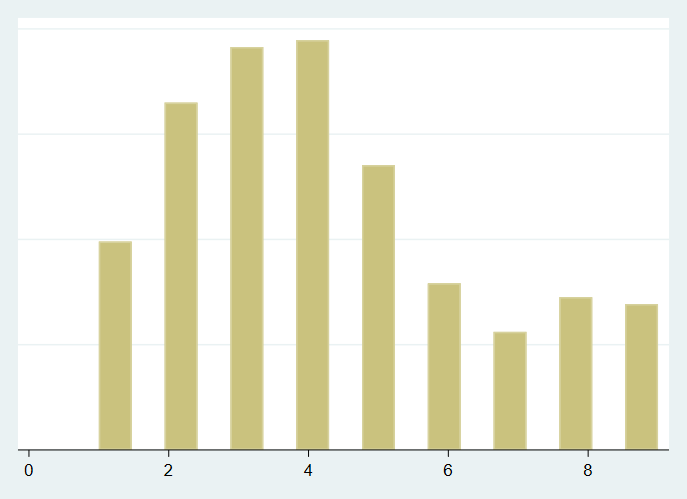
\includegraphics[width=0.8\textwidth]{./figures-and-tables/firm-size-hist.png}};
        \node (n2) [above=0.25cm] at ($(n1)!0.5!(n1) - (5.75, 0)$) {\textbf{Density}};
        \node (n3) [above=0.25cm] at ($(n1)!0.5!(n1) - (0, 4.5)$) {\textbf{Discretized Firm Size}};
    \end{tikzpicture}
    \label{fig:firm_size}
\end{figure}

Models are specified using ordinary least squares (OLS).
A robust linear model (RLM) and a generalized linear model (GLM) verify OLS results.
RLM and GLM specification alters factor significance but does not alter the coefficient value.
RLM and GLM models account for abnormal factor distribution.
In the OLS specification of Model 4, the preferred model, p-values did not exceed 0.28.
In RLM specification, p-values did not exceed 0.41.
In GLM specification, p-values did not exceed 0.38.
Overall, OLS seems slightly overfit, and RLM seems slightly underfit compared to GLM.
This analysis is mainly concerned with the direction of factor effects
rather than a precise estimate of coefficient magnitudes.
The important result from robustness testing is that coefficients did not change,
and the direction for each factor is plausible ($p < 0.5 < p'$).

Model 4 identifies seven skill gaps as important explanatory factors.
Four important skill gaps are comparative, and three are absolute gaps for ACNG candidates.
Figure \ref{fig:important_gaps} illustrates the distribution for each important skill gap.
Reflecting on this figure helps inform a diagnostic analysis for use by alternative learning providers.
ACNG candidates can also supplement their learning to address these gaps.
A simple remedy does not seem to apply for attractiveness and willingness to work odd hours.
Conscientiousness is difficult to train, but analysis suggests perception management as a remedy.
% corr cduration1 aetiwo_conscientiousness => 0.21
Perceived conscientiousness has a slight correlation duration (Pearson's $r = 0.21$).
Spending additional time to obtain a credential is a way to improve perceived conscientiousness.
ACNG supplementation of a credential with additional self-study time may also improve perceived conscientiousness.
% External research indicates that psychological therapy and other interventions can boost conscientiousness in some cases\cite{kilduff_tasselli_landis_2018}.

The important body language communication gap is an interaction with the information technology industry variable.
The interaction indicates a reduced penalty for lack of body language communication skills
in the information technology industry.
A reduced penalty for soft skill deficit helps explain the particular flourishing of
alternative credentials in the information technology industry.
The reduced penalty in this particular industry might be related to its relative lack of regulation.
Another hypothetical explanation is that the reduced penalty is related to cultural norms in the industry.
Suppose that there is a diminished technical need for social skills in programming.
In that case, introverts obtain a comparative advantage in this field.
Further study that includes personality data is encouraged to test this hypothesis.
The interacted body language skill gap and the customer service skill gap
are interesting for niche learning providers.

\begin{figure}[h!]
    \centering
    \caption{Distribution of Important Gaps}
    \begin{tikzpicture}[element/.style={minimum width=1.75cm, minimum height=0.85cm}]
        \node (n1) {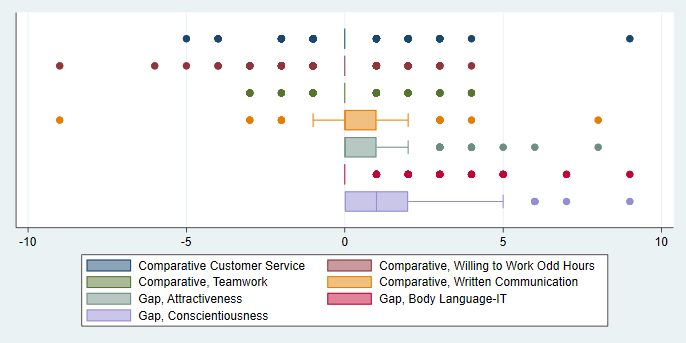
\includegraphics[width=1\textwidth]{./figures-and-tables/skill-bars.png}};
    \end{tikzpicture}
    \label{fig:important_gaps}
\end{figure}

The gaps in teamwork and written communication skill seem to be the best candidates for
feasible remedy with broad learning provider applicability.
Written communication skill is uniquely amenable to online learning.
Written communication skill is also unique in the response distribution.
The written communication skill gap is a comparative gap where the interquartile range favors ACNG labor.
This indicates the perception that ACNG providers are generally capable of providing this skill.
The distribution reflects positive and negative outliers.
Positive outliers indicate that the typical provider can improve by emulating market leaders.
Negative outliers indicate that some learning providers are particularly poor at training this skill.
If learning providers are generally effective in training this skill,
improvement for ineffective providers is likely to be feasible.

% TODO: maybe cite some literature on digital social learning or project-based learning
Alternative learning providers can use project-based learning and social learning
techniques to facilitate teamwork skill development.
These are not the most common pedagogies, but they are an established and effective pattern.
An online environment can implement courses with project-based learning and social learning.
The distribution of responses indicates that improving teamwork skill has neither the maximum
penalty nor the maximum return potential compared to improving written communication.
Model results preclude decisive prioritization of written communication skills.
Model 4 indicates that the effect of teamwork skill on hirability is more reliable
and larger in magnitude compared to the coefficient on written communication skill.
Targeting both of these two skills is feasible and beneficial to educational quality.
% where educational quality is defined as plausible impact to labor outcomes

The preferred model explains about one-third of hirability variance,
but how much of the explanatory power is attributable to skill gaps?
Table \ref{tab:explantory_power} provides evidence on the importance of perceived skill gaps and rulebreaker effects
relative to other factor groups.
Model 4 is composed of factor groups.
Table \ref{tab:explantory_power} summarizes results for simple regressions of each factor group on hirability.
Industry and state effects are factor groups regarded in external literature as important for models in the labor market.

\begin{table}
    \caption{Factor Group Explanatory Power in a Simple Regression with Hirability as Dependent Variable}
    \resizebox{\columnwidth}{!}{
        {
\def\sym#1{\ifmmode^{#1}\else\(^{#1}\)\fi}
% \begin{center}
{
    \fontsize{8pt}{7pt}\selectfont
    % \begin{small}
    \tabcolsep=3pt
    \begin{tabular}{l*{4}{c}}
        \toprule
        \multicolumn{1}{c}{Effect Group} & \multicolumn{1}{c}{Adj R-Sqr} & \multicolumn{1}{c}{R-Sqr} & \multicolumn{1}{c}{Max p-value} \\
        \midrule
        Absolute Gap                     & 0.0615                        & 0.0703                    & 0.097                           \\
        \addlinespace
        Comparative Gap                  & 0.0176                        & 0.0298                    & 0.687                           \\
        % \addlinespace
        % Rulebreaker                           & 0.1432                        & 0.1554                    & 0.053                           \\
        \addlinespace
        Industry                         & 0.0303                        & 0.0454                    & 0.958                           \\
        \addlinespace
        \addlinespace
        Other Factors                    & 0.0072                        & 0.0288                    & 0.537                           \\
        \addlinespace
        Rulebreaker                      & 0.0783                        & 0.0869                    & 0.127                           \\
        \addlinespace
        State                            & 0.0469                        & 0.1033                    & 0.772                           \\
        % \addlinespace
        % State, Semi-Robust                    & 0.0034                        & 0.0648                    & 0.831                           \\
        \bottomrule
    \end{tabular}
    % \end{center}
}
}

% TODO: maybe a count of k factors in group
% TODO: maybe distinguish strong and weak effects for industry, state, and gaps
% TODO: maybe other controls / other factors section doesn't matter
% TODO: maybe combine skill gaps

    }
    \label{tab:explantory_power}
\end{table}

Table \ref{tab:explantory_power} shows that perceived skill gaps and rulebreaker effects explain more
variance in hirability compared to the state, industry, and other effects.
Industry and state effects are also less stable.
A simple model of industry effects on hirability results in some industry effects approaching a p-value of 1.
In contrast, the least significant absolute skill gaps are statistically significant in a simple regression ($p < 0.1$).
% Rulebreaker effects collectively explain more than three times as much response variance as do industrial or state effects.
These findings collectively provide evidence that perceived skill gaps and rulebreaker
effects are factors of high importance for models of hirability.

\section{Conclusion}

% TODO: long paper food...talk about job candidate stigma mitigation techniques and hope for the ACNG
%       ACNG is not strictly dispreferred to the college grad, they just need to find a well-fitting employer
This study provides evidence that the general population is favorable to alternative credentials.
Hiring managers have higher hirability than employees that are not managers.
Alternative credentials signal a qualitatively different basket of skills compared to recent college graduates.
Americans perceive ACNG labor as weak in soft skills,
but learning providers can make changes to mitigate this issue.
Alternative credentials signal low conformity, but this results in added hirability on average.

Alternative credentials also signal that a candidate is risky.
An explanation of low ACNG demand from employer risk aversion better explains the results
compared to an explanation of selection for conformity.
In addition to a direct response indicating risk perception, firm size effects support an explanation from risk aversion.
Large employers face a lower risk premium for various reasons.
For instance, large employers can spread risk across many hires.
Risk premiums are also lower for large employers because they have access to better hiring data.

The classic signaling model explanation for employer preference of college graduate labor over ACNG labor is that
the college degree provides a comparative signal of conscientiousness and conformity.
This paper replicates the importance of conscientiousness.
Gaps in perceived conscientiousness are important,
but conscientiousness is not an important differentiator between college graduates and ACNG candidates.

While hirability is negatively associated with conformity on average, this varies importantly by the employer.
Descriptions of employer preferences better explain the willingness to hire ACNG candidates than skill gaps.
Industry effects are also important, but effects at the employer level are significantly more reliable than industry effects.
Scholars, industry members,
and others consider state effects
and industry effects to be important explanations of the willingness to hire based on an alternative credential.
Skill gaps better explain hirability compared to industry and state effects.
% Absolute skill gaps are a better explanation of hirability than comparison to recent college graduates.
% Employer factors better explain candidate hirability than do the perceived skill gaps themselves.
% Technical skill gaps explain less about hirability than soft skill gaps for ACNG job candidates.

% This paper provides evidence that some employers engage in conformity selection to avoid risk to the reputation, productivity, or value of a company.
% Ironically, such employers fail to conform to normal behavior.
% Respondents most often preferred to describe nonconformists as individuals who could just as easily be high performers as low performers.
% An explanation from risk aversion is preferred because it explains low ACNG labor demand from an employer given either of the above responses.
% Positive conformity selection is only able to explain the former case.

Risk aversion and conformity selection are both partially unconscious biases that lead to an inefficient organizational operation.
A practical recommendation is for organizations to implement bias control processes concerning ACNG evaluation.
An example of a process improvement would be for a human resources department
to maintain a list of specific credentials valued for particular job families.
% Specific criteria 
% An example improvement would be to provide human resource procedures for formal evaluation of particular credentials relevant to specified job families.
% These procedures provide immediate operational benefits regarding known credentials and job families.
% These procedures should also be retained for ongoing application as new credentials are developed and encountered over time.

Another action item is for educational institutions, policymakers, and the general public to invest further in correcting alternative education misinformation.
A survey on trade schooling taken in 2019 provides evidence on the role of this kind of misinformation\cite{arabia_2019}.
Only 27 percent of respondents correctly responded that lower debt is an advantage of enrolling in trade school relative to college.
Additionally, over 75 percent of respondents failed to notice that trade school graduates receive industry employment sooner
and receive specialized training when compared to a four-year college.
% The news that employers are generally favorable to alternative credentials should be shared far and wide.
% The current education system should be reformed to better inform students about non-college career entry.

Obtaining a college degree after obtaining some work experience will allow students to leverage employer tuition benefits.
Because ACNG hirability varies importantly by the particular employer, ACNG job candidates can reduce the risk of a lengthy job search by applying to many employers at the outset of the job search.
Social networking, online research into firm policy, and consulting with recruiters or other industry specialists are tactics to apprehend whether a particular employer is a likely member of the set that is favorable to ACNG labor.
% Government should emphasize job skills over the formal degree.
% Recent moves have begun such emphasis\cite{https://www.usatoday.com/story/news/politics/2020/06/26/trump-executive-order-stresses-skill-over-college-degree-hiring/3263074001/}

% Out of scope for this paper, but important:
% 1. aggregate social, legal, political, and economic movements (aggregate study is wanting, we know states, time, industry all matter)
% 2. applicant personal effects, and interviewer-applicant interaction effects
% despite those caveats, we can reasonably explain employer hirability their imagined candidate based on matching effects

The preferred model explains about one-third of hirability.
Perceived skill gaps and rulebreaker effects account for most of the explanatory power in the model.
There are several means of extending this research to provide improved explanatory power.
A longitudinal study would allow for causal analysis and improve forecasting of ACNG hirability in the future.
% Other research has conducted some dynamic analysis of the same dependent variable with different regressors\cite{vandivier2020preliminary}.
% Analysis that includes overqualification effects, and heterogeneous nonlinear relations between skill gaps and hirability would improve estimates of hirability for a candidate of a particular skill profile.

Firms often adopt best practices and new technologies that industry leaders first adopt.
The result that large employers and employers in the information technology industry
may indicate a future of general high support for alternative credentials.
% This paper noted that large employers and the information technology industry have a particular favorability to alternative credentials,
% but smaller firms often adopt processes and technologies which are first introduced in large f
% so recent changes implemented by Google may indicate future trends.
Google has not required a college degree since before 2013\cite{bryant2013head}.
Laszlo Bock, then Senior Vice President of People Operations at Google, stated the following in 2013:
``After two or three years, your ability to perform at Google is completely unrelated to how you performed when you were in school, because the skills you required in college are very different.''
In 2020, Google added three new certificate programs to an existing set and declared that all of its certificates are equivalent to an undergraduate degree for their hiring purposes\cite{hess_2020}.

If perceived skill represents actual skill, this study provides evidence that employers should be more willing to hire an ACNG.
At the same time, this paper provides evidence that perceived and actual skill levels sometimes do not align.
% sum aetiwno_technicaljobskills rcgtiwno_technicaljobskills
For example, the average recent college graduate in the sample has more perceived technical skills than the average ACNG.
The perceived technical deficiency among ACNG labor is surprising because last-mile training, a kind of alternative education, has been specifically recommended in popular literature to remedy the technical skill gaps among recent college graduates.
Further study of the differences between perceived and actual skills is encouraged.

In many cases, employer-perceived skill gaps are not statistically different when comparing recent college graduates with ACNG candidates.
Employers are already favorable to individuals with alternative credentials,
but specific steps will prevent the loss of this favorable status.
Results suggested curriculum improvements that target specific skills.
In addition, public education on alternative education,
the creation of new programs in underserved industries,
and public policies that give fair treatment to unaccredited education
can do much to improve public support for alternative credentials.

% Notice that the alternatively credentialed individual doesn't need the average employer to value him or her.
% He or she simply needs some significant chance of being hired, and that certainly exists.
% Moreover, the average employer is already favorable to alternative credentials.
% As more alternatively credentialed individuals are highered and promoted through society,
% there is reason to think the number of opportunities afforded to alternatively educated individuals may grow.
% The problem doesn't seem to be about whether alternative credentials work, but whether they exist in a given industrial context,
% and whether an individual would like to pay the college premium for better hirability when both options are feasible.



\chapter[Hirability and Educational Prestige]{\large Hirability and Educational Prestige}

\section{Introduction}

The accredited degree is an established means to individual-level employability, but the proliferation of the degree is associated with a variety of well-understood issues.
These issues include the student debt crisis, skill gaps, grade inflation, and low social return.
% and contribution to lack of diversity in particular labor markets.
% above, or
% and systematic demographic change to industrial labor. (which many perceive as problematic for a diverse labor pool)
Alternative credentials, or non-accredited credentials, are a broad category of offerings that exhibit greater variation intensity, price, and outcomes\cite{urdan_2020}.
Alternative credentials are often a signal of niche skills and expertise in a particular job family.
These characteristics combine to provide the benefit of high possible value addition to the labor market
with the cost of a value calculation problem shared by potential employers and education consumers.

This paper seeks to reduce the general difficulty of credential value calculation by testing a method of value normalization
with heuristics to identify those credentials likely to yield meaningful benefits to the typical job search.
This paper tests the lens of prestige as a tool to normalize value across accredited and alternative credentials.
This study leverages an original questionnaire to identify prestige levels of various credentials.
This paper tests the composite hypothesis that some level of prestige allows an alternative credential to compete with traditional credentials for employment.

Several specific lines of evidence are required to support the composite hypothesis.
Statistical evidence must demonstrate significant positive effects for accreditation and prestige on hirability.
The effect size for prestige must be sufficiently large to dominate the accreditation effect over the attainable range.
The questionnaire allows a prestige response on a 10-point scale, so the attainable range is from 1 to 10.
A vignette analysis can test whether a dominant range for prestige exists within the attainable window.
An ideal result would further show that one or more actual alternative credentials fall into this dominant range.

The motivation for the lens of prestige extends from the academic work in education economics and the economics of social norms.
Education economics provides two mainstream accounts of the value of a degree.
One account is the human capital model, and the other is the signaling model.
The human capital model explains that improved labor outcomes result from skills gained by a student in the course of education.

Stakeholders of various kinds prefer alternative credentials to the traditional degree for the attainment of specific technical skills\cite{craig2018new}.
For this reason, many college graduates supplement using alternative credentials.
Some alternative learning providers specifically target this market with a special kind of alternative education called last-mile training.
This presents an explanatory problem for the human capital model.
If better labor outcomes arise from skill enhancement,
then alternatively educated individuals should enjoy better wages, employment rates, and so on,
compared to college graduates.

The signaling model holds that credentials signal a basket of applicant qualities that employers value.
Proponents of the signaling model commonly argue that the college degree signals intelligence,
work ethic, and conformity\cite{caplan_2012}.
The signaling model presents an explanation for
the correlation of weak labor outcomes and alternative credentials,
even if alternative credentials endow students with better skills.
The explanation is that the alternative credential signals
an offsetting deficit of some kind.
This paper treats prestige as a signal rather than a matter of human capital.
This paper prefers the signaling approach to directly investigate prestige effects
with minimal theoretical baggage and without a need to test student skill.
% without concern for testing skill differences in students of various kinds.
% This paper hypothesizes that employers value prestige as a signal.
% Accredited degrees 
% A full description of such signal deficits is irrelevant to this study,
% but potential negative signals may include a deficit in conformity or work ethic.
% This study uses the signaling model as a framework for investigation
% because it appears 

% This paper hypothesizes that prestige is valued by employers as a signal.
% Prestige can be taken as a signal of conformity in part.
% Google is a prestigious employer and also an alternative learning provider.
% From the point of view of Google, their own credential is a preferred conformity signal as well as a signal of skill.
% The case of employer-provided credentials is interesting,
% but the component of prestige is 
% The main argument is that accreditation signals prestige,
% but there
% The simple hypothesis is that accredited degrees obtain higher prestige on average,
% but 
% While conformity and prestige intersect at times,
% this paper does not suppose they are identical nor generally correlated.
% Instead, this paper argues that these are two social characteristics that are valued by employers
% and a lack in one may be compensated for by the presence of the other.
% This paper hypothesizes that alternative credentials will have low average prestige,
% but that some particular credentials from prestigious providers like Google will prove valuable.

In a broad review of economics and norm types, hiring decisions exist within what Elster would identify as work norms\cite{elster1989social}.
Elster supports a rational model of work norms, with the caveat that social interactions may involve unobserved emotional effects.
Similarly, the rational model used in this paper may not extrapolate with accuracy into abnormal emotional situations.
This paper will also make use of the distinction between social and legal norms provided by Elster.

Rivera is one scholar within the economics of work norms to have recently operationalized social norms as prestige\cite{rivera2016pedigree}.
Rivera finds that prestige is important in her analysis, but her analytical scope focuses on traditional education and a few specific industries, including health and law.
The current paper extends the analysis of prestige and hiring norms
across many industries and to include alternative credentials.
% arguably I emphasize coding bootcamps / other bootcamp industries / information technology industry and perhaps sales

% To preview results,, statistical evidence confirms that prestige independently explains hirability better than accreditation alone,
% but accreditation fails to be explained away.
% Instead, models that use both factors produce superior estimates of willingness to hire.
% The independent importance of accreditation indicates that asymptotic improvements to alternative credentials are unlikely to totally outcompete the traditional education system.
% The failure of arbitrary technical and social gains in alternative credentials to fully crowd out traditional education
% points to a need to investigate legal norms for further remedy.
% The conclusion describes industry and policy solutions for the remainder of concerns in higher education.
% At the same time, there is a large level of economic value/arbitrage to be had/exploited from the socialization of alternative credentials
% before the binding constraint of legal stability is encountered.
% TODO: maybe estimate the level of economic growth (it would be proportional utility growth which is merely analgous tho)

\section{Description of Data and Methodology}

This paper investigates an original set of online questionnaire responses ($n = 454$).
Responses are cross-sectional data obtained in March of 2021.
Respondents are United States citizens at or over the age of eighteen.
Qualified respondents participated in the survey through the Amazon Mechanical Turk platform.

Appendix B contains the wording and response options for each question.
Appendix B also contains the wording for a priming message presented at the start of the survey.
The priming message lays out the definition of alternative credentials used in this study.
The message also provides several concrete examples of alternative credentials,
including ``a Certified Project Manager certification,
a portfolio of work, a Khan Academy profile, or a Nanodegree from Udacity.''

The dependent variable of interest is called hirability.
This variable measures individual response on a 10-point scale to the question,
``For many professions, alternative credentials can qualify a person for an entry-level position.''
The questionnaire is composed of three sections.
The first section collects respondent characteristics and baseline hirability.
The second section collects prestige responses with respect to nine real-world learning providers.
The third section collects hirability and prestige responses with respect to eight vignette learning providers.

% TODO: maybe describe real-world learning provider selection criteria here.

Investigation of the first section of the questionnaire uses ordinary least squares analysis.
Vignette data is analyzed as a panel in mixed models with individual random effects.
The vignette model allows comparison between prestige and accreditation coefficients.
Vignette analysis encounters a practical utility problem in that the schools are only vignettes rather than actual learning providers.
A comparison of descriptive statistics across vignettes and actual schools addresses this concern.

Half of the respondents randomly received an informational message about the nine real-world learning providers.
Appendix B includes the wording of this message.
The message provides rating data from two leading credential aggregator websites.
University ratings are US News ranking information for the 2021 school year.
Course Report provides the rating data for so-called coding bootcamps as of December 2020.

As an aside, inaccurate credential category labels contribute to the knowledge and value calculation problems that inhibit social adoption.
Coding bootcamps focus on roles in the information technology industry, but these roles are much broader in scope than the category label implies.
Moreover, the information technology industry is a special industry that cuts across all other industries.
Much of the academic, policy, and industry discussion on coding bootcamps misses that these institutions provide credentials that potentially compete with university degrees in nearly any subject.

For example, General Assembly is one of the particular coding bootcamps investigated in this study.
General Assembly provides credentials for user experience design, a set of skills involving market research, and applied technical art skills.
General Assembly provides credentials for product management.
Product management is a job family that competes for labor among business degree graduates.
The data science credential provides skills that compete with accredited labor in mathematics, statistics, economics, and even subjects in the hard sciences like computational biology.
Finally, there are credentials that relate to software development and compete with accredited degrees in computer science.

% TODO: write the below content into the paper when we get to results on concrete providers
% why do we not use a mixed model of concrete providers?
% three reasons:
%   first, the whole point of using an aggregator is to obtain individual-independent data
%   second, ratings are heterogenous so there would be some noise introduced by indexing them together
%   third, i use stipulated prestige categories as a pseudo-index
%       the pseudo-index can be used via simpler descriptive stats,
%       and the pseudo-index has evidence supporting it; that is, high / low stipulated prestige is sig correlated to response prestige.
% if all those objections fail, then fine we can do it but i suspect the answer will be:
%   'findings are insignificant bc of low variation and injected noise not bc no such level exists'

Respondent characteristics are categorical variables.
Hirability and prestige are 10-point Likert-type responses.
Prestige takes a second representation as a stipulated boolean.
Stipulating prestige enables the application of results to a real job search.
If stipulated prestige is highly correlated to prestige response,
and if prestige response is correlated to improved hirability,
then the selection criteria for stipulated prestige can be applied in an actual job search to potentially improve outcomes.

To illustrate the method of two-way prestige validation,
suppose that a vignette school is stipulated as high prestige.
This situation is represented in regression as a dummy variable for stipulated high prestige with a value of true.
The respondent reads that the vignette school is known to be prestigious.
After reading this, the respondent provides a prestige response rating on a 10-point scale.
Investigation of all responses allows an analyst to determine an average prestige response level which is associated with
the stipulated high prestige criteria.

To preview results, stipulated high prestige turns out to be strongly correlated with high prestige response.
Interestingly, there are cases where a respondent gives a low response rating to, for example,
the University of Chicago, a school with high stipulated prestige based on aggregator website ratings.
This result indicates the importance of some analysis that accounts for individual effects.
% the person could just be generally stingy with hirability points, they might be particularly opposed to accredited degrees, have a special issue w this school...

Two-way representation of prestige enables the application of findings into an actual job search.
In an actual job search, individuals can easily access aggregator website data.
In the real world, an individual cannot readily access questionnaire results for many credentials.
Results from this paper include the identification of rules of thumb
that a person can use to identify actual learning providers as high prestige.
To ensure clarity of results, stipulated prestige always refers to the dummy variable, and prestige response refers to the 10-point measure.

The vignette section and the section on actual schools use stipulated prestige.
All other variables are either 10-point Likert-type responses or categorical variables\footnote{
    It is an accepted practice to treat Likert-type responses as either categorical or continuous for regression analysis.
    Jaccard and Wan provide support for continuous analysis of Likert-type data.
    They note that severe departures from the assumptions on cardinality ``do not seem to affect Type I and Type II errors dramatically,''
    particularly when the Likert scale is five or more points\cite{jaccard1996lisrel}.
    This paper treats responses on a 10-point scale as continuous.
}.
Categorical variables are exclusively respondent characteristics.
Four other respondent measures are Likert-type responses.
Vignette responses include responses for hirability and prestige,
while actual schools only receive responses for hirability.
% Prestige is measured two-ways in the vignette section, but it is only stipulated in the section on actual schools.

Respondent characteristics include eight standard controls and four questions unique to this study.
The eight standard controls include
age, gender, ethnicity, income,
level of education, employment status, the industry of occupation, and state of residence.
A unique question on work norms records whether the respondent tends ``to work more closely with coworkers at your company or customers and external business partners.''
The motivation for this question is to test whether prestige disproportionately impacts roles that are outward or client-facing.
Respondents are also directly asked whether they
``prefer to hire or work with a person that has a college degree rather a person that holds a reputable certification or non-college credential.''

Another unique control is support for online education.
This control allows analysis to separate hirability effects due to online education preference
from hirability effects due to unaccredited education preference.
In practice, many alternative credentials involve online learning,
but accredited learning is also increasingly taking place online.

The fourth control is expected conventionality.
% This is an important representation of perceived social norms.
This variable measures whether the respondent believes that
``It will soon become common for high school graduates to obtain alternative credentials instead of going to college.''
This is a useful correction variable for two reasons.
First, it separates willingness to hire based on respondent preference
from indirect willingness to hire based on perceived social norms.
Individual preferences and social norms are certainly correlated,
but the correlation is small enough that failure to separate these effects leads to nontrivial statistical noise.

Second, surveys sometimes overreport demand effects because of the lack of cost constraint on respondent expression.
This bias is sometimes called budget constraint bias or omitted budget constraint bias\cite{ahlheim1998contingent, pachali2020omitted}.
% This is also in part corrected for by collecting income...so there isn't an 'unobserved budget' really...see sources cited
Without a cost constraint, respondents tend to exaggerate demand responses like the willingness to hire.
Budget constraint bias affects both hirability and expected conventionality,
so conventionality operates in part as a bias control.

Vignette question formatting follows Atzm{\"u}ller and Steiner\cite{atzmuller2010experimental}.
Each vignette stipulates whether a school is accredited,
whether the respondent should imagine the school as impressive,
and whether the respondent should imagine that other people consider the school impressive.
Each stipulated factor can take a value of true or false,
resulting in eight vignette questions.

This study uses multiple regression and descriptive statistics to generate results.
% \footnote{
%     While the data for this analysis is not public, the analytical code is open-source.
%     See \url{https://github.com/Vandivier/research-dissertation-case-for-alt-ed/tree/master/papers/alt-ed-prestige}
% }.
Multiple regression is conducted using ordinary least squares (OLS)
for baseline hirability analysis
and linear mixed models (LMM)
are used for vignette analysis.
OLS specification of vignette data is inappropriate because repeated measures of hirability
from a single participant introduce an individual-level bias into resulting coefficients.
LMM models are able to account for these individual-level effects.
Following Magezi\cite{magezi2015linear},
linear mixed models in this paper use a within-participant random factor,
or individual random effects,
to correct for individual-level repeated measures bias.
LMM yields linear coefficients, so the interpretation of LMM coefficients is similar to OLS.
One difference of note is that adjusted r-squared is not available for an LMM model.
% For this reasons, an OLS model is optimized for baseline hirability,
% and then that specification is trivially modified into an LMM model for further analysis.
% formula for LMM at https://www.statsmodels.org/stable/mixed_linear.html
% individual random effects https://www.statsmodels.org/stable/examples/notebooks/generated/mixed_lm_example.html#Growth-curves-of-pigs

% 2. how was nonresponse bias addressed? - maybe not at all
% - main way to address nonresponse bias is to explicitly capture and correct for all of the individual characteristics that matter: ethnicity, age, income...
% - it would not be enough to show nonresponse bias exists;
% - it would need to be shown that it exists in the direction of some effect that moves the relation of interest in a predictable and meaningful way;
% - else the criticism is an argument from ignorance which due dilligence has been undertaken to preclude.
% - https://forum.effectivealtruism.org/posts/a6LMQcER6Awhawtqq/using-amazon-s-mechanical-turk-for-animal-advocacy-studies
% - above indicates overstatement of effects...i would want more info...there is a paper internally cited
% - above also deflates income nonresponse bias consern (these don't pay much so systematic bias from rich ppl) also i explicitly capture income anyway
% - "AMT was found to be a reliable source of data and to diminish the potential for non-response error in online research"
% - https://www.ncbi.nlm.nih.gov/pmc/articles/PMC4397064/
% - https://duckofminerva.com/2013/07/mechanical-turk-and-experiments-in-the-social-sciences.html
% - https://www.tandfonline.com/doi/abs/10.1080/10967494.2016.1276493
% 3. How were ratings subjects selected? min 2*2*2 (isQuality)*(isBootcamp)*(isKnown) social and individual ratings [10 point likert-type unit]
% 4. a few correction variables based on literature review and computed norm factors how

\section{Results}

% top line results; alt creds are lower prestige on average but still important
Results ($n = 454$) indicate that accredited degrees are generally higher in prestige compared to alternative credentials.
Alternative credentials are meaningfully associated with hirability,
and in certain situations, they are preferred to accredited degrees.

Competitive status indicates that a credential is correlated with hirability to a similar or greater extent compared to an accredited degree.
Results provide evidence for three cases in which alternative credentials are competitive.
First, specific alternative credentials are of particularly high prestige.
This study finds that a credential from Google is sufficiently prestigious to be competitive without a requirement of supplementary conditions.

Second, some individuals award prestige preferentially to alternative learning providers.
% analysis_5_transfer table a5.1
In a comparison among nine actual learning providers in this study,
71 percent of respondents prefer at least one alternative credential to at least one university degree.
The proportion increases to about 75 percent when respondents view rating data from the online review aggregators Course Report and US News.
% These sites include US News and Course Report, and they aggregate learning providers,
% report standard information about those providers,
% and allow users to leave reviews.

% TODO: maybe re-introduce the term 'alternativel credentialed non-college graduated' / ACNG.
Third, certain independent factors in hiring decision models support the hirability of alternatively credentialed job candidates.
Industry and state effects are two such compensating factors that can add up to overcome the average comparative preference for accredited labor to alternatively credentialed job candidates.
% For example, the state effect for California is positive on hirability
% and it retains a magnitude that compensates almost exactly for the hirability penalty from non-accreditation.

% summary statistics
% a2.1
Baseline hirability is the institution-agnostic hirability measure.
The mean response for baseline hirability is 7.58 on a 10-point scale, and the median response is 8.
Table \ref{tab:desc_stats} gives average hirability and prestige for interesting segments of respondents.
Four basic results in the table are worth noting.
First, stipulated prestige always moves with prestige response as expected.
Second, as expected, the hirability and prestige effects for accredited schools are generally higher than non-accredited schools.

Third, the difference in average hirability between high and low prestige providers
is more than twice the difference in hirability between accredited and unaccredited providers.
This supports the possibility of an actual competitive alternative credential in the attainable range of prestige.
% alternative education becomes competitive with traditional education.
% The fourth result is that the average actual school with stipulated high prestige
% is too low in prestige to be competitive with the average actual school with an accredited status.
The fourth result is an initial attempt at a prestige rule of thumb.
For both vignette and actual schools,
if a school can obtain a prestige score of 7 or more,
it will be at least as prestigious as the average accredited school.

\begin{table}
    \caption{Average Hirability and Prestige}
    \resizebox{\columnwidth}{!}{
        {
\def\sym#1{\ifmmode^{#1}\else\(^{#1}\)\fi}
\begin{tabular}{llcc}
    \toprule
                              &                                   & \textbf{Average Hirability} & \textbf{Average Prestige} \\
    \midrule
    \textbf{Actual Schools}   &                                   &                             & 6.50                      \\
                              & \textbf{Accredited}               &                             & 7.05                      \\
                              & \textbf{Unaccredited}             &                             & 6.07                      \\
                              & \textbf{Difference}               &                             & 0.98                      \\
    \cmidrule{2-4}
                              & \textbf{Stipulated High Prestige} &                             & 6.72                      \\
                              & \textbf{Stipulated Low Prestige}  &                             & 6.23                      \\
                              & \textbf{Difference}               &                             & 0.49                      \\
    \cmidrule{2-4}
    \textbf{Vignette Schools} &                                   & 6.49                        & 6.21                      \\
                              & \textbf{Accredited}               & 6.97                        & 6.49                      \\
                              & \textbf{Unaccredited}             & 6.02                        & 5.93                      \\
                              & \textbf{Difference}               & 0.95                        & 0.56                      \\
    \cmidrule{2-4}
                              & \textbf{Stipulated High Prestige} & 7.59                        & 7.69                      \\
                              & \textbf{Stipulated Low Prestige}  & 5.63                        & 4.94                      \\
                              & \textbf{Difference}               & 1.96                        & 2.75                      \\
    %   \midrule
    % \textbf{Pooled}           &                                   &                             & 6.37                      \\
    %                           & \textbf{Accredited}               &                             & 6.77                      \\
    %                           & \textbf{Unaccredited}             &                             & 6.01                      \\
    %                           & \textbf{Difference}               &                             & 0.76                      \\
    %                           & \textbf{Stipulated High Prestige} &                             & 7.00                      \\
    %                           & \textbf{Stipulated Low Prestige}  &                             & 5.80                      \\
    %                           & \textbf{Difference}               &                             & 1.20                      \\
    \bottomrule
    \bottomrule
\end{tabular}
}

    }
    \label{tab:desc_stats}
\end{table}

% The differences reported in Table \ref{tab:desc_stats} are significant ($p < 0.1$).
% Smaller differences between actual schools and vignette schools are also significant.
% The minimum difference of 0.14 between unaccredited actual and vignette schools is significant ($p < 0.1$).

Google is the only unaccredited learning provider to achieve a competitive status on the basis of this initial rule.
The mean prestige response for Google was 7.10, and the median response was 7.
Two lower bars for competitive status are interesting.
First, an alternative provider can be described as moderately competitive if it fails to beat the average university,
but it succeeds in beating at least one university on average.
The lowest average prestige response for an accredited university is 6.34 for the University of Nebraska.

Second, an alternative provider can be described as weakly competitive if it fails to beat any university on average,
but it succeeds in beating at least one university in a significant percentage of individual responses.
No alternative credentials investigated in this study meet the criteria for moderate competitiveness.
App Academy, General Assembly, and Google are the three alternative learning providers with stipulated high prestige.
All stipulated high prestige learning providers are at least weakly competitive.

When asked directly, 41.6 percent of respondents indicated that they would not prefer to
work with a person that holds an accredited credential instead of ``a person that holds a reputable certification or non-college credential.''
When examining prestige response instead of asking directly, over 70 percent of respondents reveal a preference for
at least one actual alternative credential to at least one university credential.
Over half of respondents preferred at least one actual alternative credential with stipulated high prestige
to at least one university credential with stipulated high prestige.
After excluding Google, over one-quarter of respondents continue to prefer
at least one actual alternative credential with stipulated high prestige to at least one university credential with stipulated high prestige.

% TODO: Does zety belong in the conclusion?
Zety is an online platform that facilitates job search.
Zety reports that one in six job applicants in the United States receive an interview,
and the average conversion rate from interview to offer was 19.78 in 2016\cite{turczynski_2021}.
Assuming rejections are independent enables naive estimation that most job searches consist of at least four interviews\footnote{
    Four independent games that each include an eighty percent chance of rejection yields $0.8^4 = 0.4096$.
    The associated probability of having at least one offer result from four interviews would be about $1 - 0.41 = 0.59$,
    or 59 percent, which is more likely than not.
} and dozens of applications.
Given the rates at which respondents prefer alternative credentials to accredited degrees,
a job search of typical length is likely to include several applications and at least one interview
with one or more employers that would prefer an alternative credential with stipulated high prestige to an accredited degree.

% More than half of respondents prefer a high prestige alternative credential to at least one high prestige accredited degree.
% After excluding the highest prestige alternative credential from Google,
% more than one-quarter of respondents still prefer one of the remaining high prestige alternative credentials to at least one high prestige accredited degree.
% % a2.2
% When asked directly, about 42 percent of respondents state that they do not prefer
% to work with a person that has a college degree rather than a person that holds a reputable non-college credential.

{
\def\sym#1{\ifmmode^{#1}\else\(^{#1}\)\fi}
\begin{center}
    {
        % \fontsize{8pt}{7pt}\selectfont
        \tabcolsep=2pt
        \begin{longtable}{l*{3}{c}}
            \caption{Table of Regression Results}
            \label{tab:table_regs}                                                                                                       \\

            \toprule
                                               & \multicolumn{1}{c}{Model 1} & \multicolumn{1}{c}{Model 2} & \multicolumn{1}{c}{Model 3} \\
            \midrule
            \endfirsthead

            \multicolumn{4}{c}%
            {{\bfseries \tablename\ \thetable{} -- Continued}}                                                                           \\
            \addlinespace
            \toprule
                                               & \multicolumn{1}{c}{Model 1} & \multicolumn{1}{c}{Model 2} & \multicolumn{1}{c}{Model 3} \\
            \midrule
            \endhead

            \addlinespace
            \hline
            \multicolumn{4}{|c|}{{Continued on Next Page}}                                                                               \\
            \hline
            \endfoot

            \hline \hline
            \endlastfoot

            % \hline
            %                                    & Model 1 & Model 2  & Model 3  \\
            % \hline
            Age, 45-60                         & 0.61***                     & 0.10                        &                             \\
            % \addlinespace
            External Facing, High              & 1.23***                     & 0.13                        &                             \\
            External Facing, Low               & 1.16***                     & 0.10                        &                             \\
            External Facing, Medium            & 1.16***                     & 0.13                        &                             \\
            Expected Conventionality           & 0.32***                     & 0.14***                     & 0.17***                     \\
            Income, 0-9999                     & 0.88                        & -0.87**                     & -1.22***                    \\
            Income, 100,000-124,999            & 1.25***                     & 0.47**                      & 0.41*                       \\
            Income, 175,000-199,999            & 1.58*                       & 0.40                        &                             \\
            Income, 200,000+                   & 1.14                        & -1.09*                      &                             \\
            Income, 25,000-49,999              & 0.57**                      & 0.19                        &                             \\
            Income, 50000-74999                & 0.51**                      & 0.26*                       & 0.18                        \\
            Income, 75000-99999                & 0.81***                     & 0.29*                       &                             \\
            Industry, Education                & 0.66**                      & 0.40**                      &                             \\
            Industry, Finance                  & 0.34                        & -0.07                       &                             \\
            Industry, Information Technology   & 0.46**                      & 0.05                        &                             \\
            Industry, Manufacturing            & 0.34                        & 0.17                        &                             \\
            Industry, Other                    & 0.37                        & 0.37**                      &                             \\
            Is Accredited                      &                             & 1.23***                     & 1.27***                     \\
            (Is Accredited)(Prestige Response) &                             & -0.09***                    & -0.10***                    \\
            Is Stipulated High Prestige        &                             &                             & 0.14**                      \\
            Is Stipulated Other Impressed      &                             & 0.64***                     & 0.59***                     \\
            Is Stipulated Self Impressed       &                             & -0.05                       &                             \\
            Online Ed Favorability             & 0.34***                     & 0.09***                     & 0.07**                      \\
            Prefers Traditional Coworker       & -0.22                       & 0.19*                       & 0.19*                       \\
            Prestige Response                  &                             & 0.55***                     & 0.53***                     \\
            State, Arizona                     & 1.35**                      & 0.69**                      &                             \\
            State, California                  & 0.44**                      & 0.27**                      & 0.37**                      \\
            State, Connecticut                 & 0.72                        & -0.11                       &                             \\
            State, Florida                     & 0.79***                     & 0.16                        &                             \\
            State, Georgia                     & -0.88*                      & -0.22                       &                             \\
            State, Kansas                      & 1.76                        & 0.52                        &                             \\
            State, Maryland                    & 0.92**                      & 0.31                        &                             \\
            State, Massachusetts               & 1.43**                      & 0.49                        &                             \\
            State, Michigan                    & 1.35***                     & 0.26                        &                             \\
            State, Mississippi                 & 1.77***                     & 0.45                        &                             \\
            State, Missouri                    & 0.81*                       & 0.34                        &                             \\
            State, Nebraska                    & -1.04                       & -0.75                       &                             \\
            State, New Mexico                  & 1.76*                       & 0.10                        &                             \\
            State, Pennsylvania                & 0.44                        & 0.44**                      &                             \\
            State, Tennessee                   & 0.74                        & -0.13                       &                             \\
            State, Texas                       & 0.39                        & -0.10                       &                             \\
            State, West Virginia               & -1.31                       & -0.92                       &                             \\
            Intercept                          & 0.30                        & 0.14                        & 0.50*                       \\
            % \hline
            \midrule
            R-squared                          & 0.47                        &                             &                             \\
            R-squared Adj.                     & 0.42                        &                             &                             \\
            N                                  & 454                         & 3600                        & 3600                        \\
            Measures Per Respondent            & 1                           & 8                           & 8                           \\
            % \addlinespace
            % Constant                         & 5.036\sym{***}        & 5.356\sym{***}        & 4.755\sym{***}     \\
            % \midrule
            % Adjusted R-sqr                   & 0.2181                & 0.2512                & 0.2331             \\
            % R-sqr                            & 0.3253                & 0.3539                & 0.3310             \\
            % p(F)                             & 0.0000                & 0.0000                & 0.0000             \\
            \hline
            % \addlinespace
            \multicolumn{4}{l}{\footnotesize \sym{*} \(p<0.10\), \sym{**} \(p<0.05\), \sym{***} \(p<.01\)}                               \\
        \end{longtable}
    }
\end{center}
}


Table \ref{tab:table_regs} gives three models.
The first model is an ordinary least squares model of baseline hirability.
Backward elimination to the point of adjusted r-squared maximization yields Model 1.
Adding factors of accreditation and prestige to Model 1,
then adapting the model to a linear mixed model (LMM) yields Model 2.
Model 3 results from additional backward elimination on Model 2.

Four individuals that completed the first section of the questionnaire
did not complete the entire questionnaire.
The remaining 450 respondents each report hirability for the eight vignette schools,
yielding 3,600 observations for the mixed models.

Because LMM does not permit computation of r-squared,
the termination criteria for the factor elimination process in Model 3
was to retain all factors with a p-value under 0.5.
This is a permissive criterion intended to guard against overfitting.
The logical basis for this rule is that each observed effect is
more likely to exist than to not exist when $p < 0.5$.
Despite permissive criteria, only one insignificant factor for income exists in Model 3.

% Comparison of coefficients across specifications improves confidence in the coefficients in all but two cases.
% The factor for the income range under ten thousand dollars per year
% and the factor for preference in a traditional coworker flip signs,
% but other factors are fairly consistent in their effects.

Model 2 and Model 3 have one other interesting difference.
Model 3 includes the boolean for whether a school was stipulated as high prestige.
For vignette schools with high prestige, the participant viewed two statements about the vignette.
The questionnaire instructs the participant to imagine a school they consider to be impressive.
The questionnaire also instructs the participant to imagine that other people consider the school to be impressive.
This situation is technically equivalent to an interaction of the two subcomponents.
Because Model 2 includes both stipulated high prestige subcomponents and the accreditation dummy, including high prestige generates perfect multicollinearity.
Backward elimination of Model 2 drops the factor for own stipulated prestige, so subsequent insertion of high prestige is nonproblematic.

Model 3 is the preferred model.
Prestige and accreditation effects are positive and significant.
These two effects also interact with a significant and negative coefficient.
The values of these coefficients of interest are consistent across Model 2 and Model 3.
The dummy variable for accreditation is about two and a half times larger than the prestige response,
but the average prestige response is near seven.
This indicates that the prestige response explains a larger share of hirability variance compared to accreditation.
% The negative interaction indicates both a decreasing marginal benefit for prestige among the accredited,
% and also a decreasing marginal penalty for prestige among the unaccredited.

An application of Model 3 is another approach to the identification of competitive alternative credentials.
Hold factors other than accreditation and prestige constant.
Let the hirability level of school $k$ be called $H_k$.
Let $X_{ka}$ be accreditation status,
$X_{kp}$ is prestige response,
$X_{kh}$ is the dummy for stipulated high prestige,
and $X_{ko}$ is the dummy for whether other people consider the school prestigious.

Let $H_1$ be an unaccredited school with high stipulated prestige.
Let $H_2$ be an accredited school without high stipulated prestige.
% Let $H_2$ receive a prestige response equal to the average for an accredited vignette.
Let $X_{2p} = 6.49$, which is the prestige response equal to the average for an accredited vignette,
as reported in Table \ref{tab:desc_stats}.
This system of equations is described in equations \ref{eq1} through \ref{eq5}:

\begin{subequations}
    \begin{equation}
        H_k = 1.27X_{ka} - \num{0.1}X_{ka}X_{kp} + 0.53X_{kp} + 0.14X_{kh} + 0.59X_{ko}
        \label{eq1}
    \end{equation}
    \begin{equation}
        H_1 = 0.53X_{kp} + 0.14 + 0.59
        \label{eq2}
    \end{equation}
    \begin{equation}
        H_2 = 1.27 - \num{0.1}(6.49) + 0.53(6.49)
        \label{eq3}
    \end{equation}
    \begin{equation}
        X_{kp} = (1.27 - \num{0.1}(6.49) + 0.53(6.49) - 0.14 - 0.59) / 0.53
        \label{eq4}
    \end{equation}
    \begin{equation}
        X_{kp} \approx 6.28
        \label{eq5}
    \end{equation}
\end{subequations}

Equation \ref{eq5} indicates that an alternative credential
with stipulated high prestige
and a prestige response of 6.28 or higher is approximately competitive with the average accredited vignette.
Table \ref{tab:desc_stats} indicates that the prestige response for the average vignette school is 6.21.
This is a significant difference compared to the average actual school prestige response of 6.50.
Coincidentally, additive and proportional compensation of 6.28 both yield 6.57.

This prestige requirement exceeds the low bar set by comparison to the University of Nebraska.
Google remains the only alternative provider to obtain general competitive status without the presence of other preferential factors.
App Academy and General Assembly both have average prestige responses close to 5.8.
Models reveal several situations in which other factors overcome this deficit,
but many of these offsetting factors are difficult to determine and leverage prior to a hiring decision.
The California state effect is an interesting exception that an actual job search could exploit.

Alternative credentials provide a source of potential diverse labor to employers.
Interestingly, neither ethnicity nor gender was significantly associated with hirability.
There is little evidence for the thesis that client-facing roles preferentially benefit from credential prestige or accreditation.
Respondent client exposure on the job was associated with a slightly larger baseline willingness to hire an alternatively educated candidate.
The extent of client contact was insignificant in mixed models.

\begin{figure}[h!]
    \centering
    \caption{Prestige Response Distribution for Actual Schools}
    \begin{tikzpicture}[element/.style={minimum width=1.75cm, minimum height=0.85cm}]
        \node (n1) {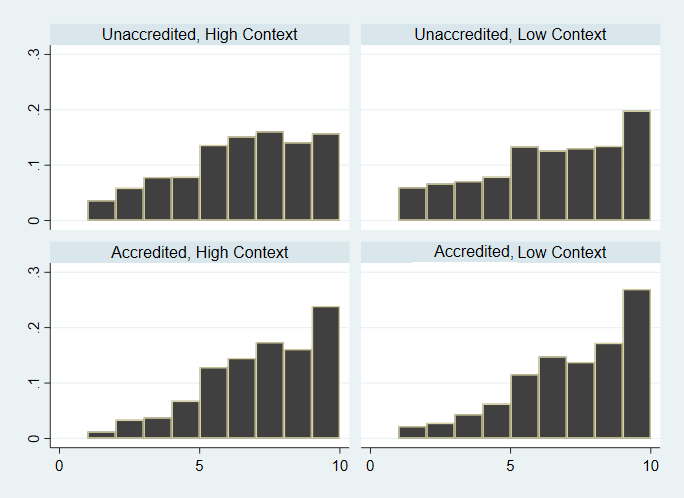
\includegraphics[width=1\textwidth]{./figures-and-tables/context-graph-massaged.png}};
    \end{tikzpicture}
    \label{fig:var_results}
\end{figure}

% This effect does not enter in to any regression
Finally, Figure \ref{fig:var_results} visualizes the prestige response distribution
for actual schools.
The four subplots describe whether a respondent randomly received information from review site aggregators
and how they evaluated credential accreditation.
Exposure to aggregated review information is associated with fewer responses at the positive
and negative extrema of the response distribution for accredited and unaccredited schools.
On average, alternative education prestige rose,
and accredited education prestige declined when a respondent received review aggregator site information.

\section{Conclusions}

This study hypothesized that some level of prestige allows an alternative credential to compete with traditional credentials for employment.
Results provide evidence in favor of this hypothesis.
Regression results show meaningful positive correlations of prestige and accreditation on hirability.
A range of hirability responses that include the average response and some below-average responses
find a dominant explanation in prestige effects over accreditation alone.

While prestige explains a larger share of hirability variance than accreditation, accreditation robustly maintains a meaningful effect on its own.
The robust importance of accreditation indicates that arbitrary improvements to alternative credential
quality and social acceptability are not likely to displace the higher education system in expectation.
This study began with the assertion that alternative credentials are a source of unexploited technical value.
The study validated a partial explanation from prestige as a representation of social norms.
The introduction noted an important distinction between legal and social norms from Elster.
By elimination, legal norm change is an important candidate to allow alternative credentials the opportunity
to fully outcompete the hirability effects of accreditation.

% While prestige explains a larger share of hirability variance than accreditation,
% accreditation robustly maintains a meaningful effect on its own.
% The robust importance of accreditation indicates that arbitrary improvements to alternative credential
% quality and social acceptability are not likely to displace the higher education system in expectation.
% % quality and social acceptability will not displace the higher education system in expectation.
% % quality and social acceptability will not displace the higher education system in expectation.
% Synthesis of the distinction from Elster between social and legal norms with the results of this study
% point to a need for legal norm change in order to create a competitive environment between traditional and alternative providers.
% % A change in legal norms appears to be required in order to create an even competitive environment between traditional and alternative providers.

In 2012, The Heritage Foundation called for two policy changes that are worth considering.
First, the Foundation proposed that the government should directly accredit courses rather than organizations\cite{burke2012accreditation}.
Second, they also called for a decoupling of accreditation and federal funding.
An additional option would be to replace legal requirements for formal education could be replaced with skill assessments.
With a legal requirement that prefers skills to degrees,
the public sector gains the ability to transfer formal accreditation duties to a market model with no loss of labor quality control.

There are several reasons to be pessimistic about the feasibility of these policy changes.
Reductions to education spending are unpopular with voters in the United States.
% Education is compulsory in the United States.
Over ninety percent of K-12 students in the United States attended a public school in 2016\cite{us2019digest},
and there is a systematized pipeline from public school to the traditional university system.
Education represents an example of an entangled political economy\cite{wagner2014entangled}.
Robust political economy points out additional reasons to doubt rapid innovation in this space\cite{boettke2004liberalism}.
Reduced political entanglement is associated with the absence of compulsory education.
However, after they exist, the elimination of compulsory laws also appears intractable.
The removal of compulsory education is a qualitative change that does not appear any less subject to the path dependency,
lock-in, ratchet, and other effects that inhibit contraction in the quantitative process of appropriations.
% Ratchet Effect
% One way to weaken the degree of political entanglement entanglement would be the absence of compulsory education laws,

An interesting alternative to formal legislative change is the emerging model of public-private partnerships in education.
In 2013, Georgia Tech formally partnered with Udacity to produce an accredited online graduate degree in Computer Science\cite{empson_2013}.
Udacity was able to facilitate an improved online learning experience at scale with an affordable price.
Georgia Tech offered branding, legitimacy, and accreditation, which supported a higher price point compared to the other offerings from Udacity.

In other cases, the hybridization of traditional and alternative education is indirect and informal.
Prior learning assessments and portfolio reviews are two of many processes by which a university can award credit to a student
without formal requirements connected to the source of student learning\cite{conrad2008building}.
University support for prior learning is an implementation pattern for course-level accreditation that does not require legislative action.
Formal and informal partnerships between traditional and alternative institutions can yield increased market surplus for producers and consumers.

Finally, this paper evaluated practical alternative credential selection strategies.
One strategy is to leverage credentials from industry leaders.
In this study, Google represented an alternative learning provider that is also an industry leader.
Fortune 50 membership is a rule of thumb used in this study to select an industry-leading firm.
A credential from Google was the only alternative credential to be identified as generally competitive with an accredited degree.

The second strategy is to use credential review aggregator sites to identify high prestige credentials.
This paper used Course Report as an aggregator to search for alternative credentials.
App Academy and General Assembly were identified by applying search criteria that include a rating of 4.25 or better on a 5-point scale and a minimum of four hundred reviews.
The combination of results with information on typical job search length from Zety indicated
that these credentials provide meaningful job search benefits,
albeit with significantly less efficacy than an accredited degree or a credential from Google.




\chapter[COVID-19 and Alternative Postsecondary Learning]{\large COVID-19 and Alternative Postsecondary Learning}

\section{Introduction}

Has COVID-19 pushed technology forward in education?
Online learning has become increasingly utilized since the turn of the century,
but have forced social distancing measures sparked a new disdain for remote learning?
Scholars have recently uncovered impacts in the American K-12 space and the university system,
but this paper adds much-needed attention to the question of alternative credentials
and unaccredited postsecondary education.

This study is concerned with alternative postsecondary credentials.
This category includes professional certifications, coding bootcamps, work portfolios,
and other proof of education other than traditional credentials.
In this study, traditional credentials mainly refer to the accredited college degree.
Remote learning was an alternative approach to education from inception, and it continues to be deeply involved in alternative learning.
This study hypothesizes that the impact of coronavirus is positive on favorability to alternative credentials.
Results favor the hypothesis, with evidence that exposure to remote learning is a critical mechanism.

There are three theoretical reasons to suppose that a pandemic would make alternative postsecondary credentials more attractive.
The first is that the pandemic response has resulted in exposure to remote activity,
and exposure effects are often positive on favorability.
Second, alternative learning providers face different incentives compared to traditional providers.
Differing incentives may provide an adaptive advantage in the face of rapid social change.
A recent paper on organizational agility in higher education points to regulatory challenges
and deep, centralized, hierarchical organizational structure as notable disadvantages\cite{menon2020factors}.

The third theory is that a pandemic is a time when normal strangeness increases across society.
When the normal level of strangeness increases, things that were already finitely strange become relatively less strange.
Alternative credentials are strange in some sense by construction,
but the relative stigma associated with these credentials might decrease in a time like that of the present pandemic,
where all sorts of previously strange behaviors have become a new normal.
% Suppose that a strange thing becomes less strange when it is logically explained.
% In this case, remote activity plays a logical role as a social distancing solution, 
% and benefits to favorability from remote activity are not clearly reduced to mere exposure effects.
% Moreover, any stigma associated with a person selecting cheap education becomes less of an issue
% when the logic that a pandemic causes general financial difficulty is accounted for.
% This becomes more plausible when the connection of alternative credentials to remote activity is highlighted.
% At a time when personal contact is costly,
% remote learning becomes a better bargain,
% and the social benefits of traditional education are simultaneously diminished.

% This would theoretically reduce any relative stigma which the alternatively educated invididual might face.
% The stigma is reduced by two mechanisms.
% First, society changes many norms during a pandemic, so the general strength of social norms is reduced.
% In this way, the general preference for traditional over alternative education is reduced.
% Secondly, consuming alternative education is specifically reasonable as a pandemic adaptation.
% During a pandemic, many of the attractions of university life are unusable,
% remote learning provides protection against becoming ill,
% and pinching pennies is more understandable than it is during times of flourishing.
% When an individual has such good reasons for pursuing alternative education, it becomes unreasonable to impose a stigma at hiring decision time.
% TODO: the above is related to mitigation tactics for disabled people during interview; stigma management...idk the exact keywords look it up

% The third reason that a pandemic could make a massive shift to alternative learning more reasonable
% is simply that massive shifts are less spectacular in a time of pandemic.
% Society has already changed many norms in the face of the pandemic.
% Some of these norm changes are directly linked while others are indirect.
% Social distancing, wearing masks, fewer shaken hands, and so on, are some direct measure.
% The lack of fresh bread at my local coffee shop is an indirect change resulting from supply chain cost impact of the pandemic.
% Both are understandable changes.
% In this pandemic context an empathetic employer would look at an alternatively educated individual as making a reasonable adaptation,
% whereas previously they might face some stigma for making a strange choice.
% In a time where many norms are being disrupted, there may be an external effect which weakens norms in general,
% and therefore the general preference of traditional to alternative education would.

While exposure to some stigma generally increases favorability, there are several special cases where it declines instead.
Coronavirus-induced exposure could be such a case of negative exposure for a few reasons.
Direct exposure to disease is generally harmful, unwanted, and forced.
Disease-induced activities are not strictly involuntary,
but they might be perceived disfavorably by association.
The mere exposure effect\cite{robinson2005novel} and familiarity bias\cite{cao2011fear}
are generally positive on favorability to some stimulus,
but these exposures are often voluntary.
Unwanted exposure that involves harm tends to reduce favorability.
Backfire, boomerang, and blowback effects are examples of a negative response to exposure
\cite{swire2020searching, byrne2009boomerang, campagna2016strategic}.
One study relates closely to the COVID-19 pandemic in finding a backfire effect in efforts to market flu vaccine usage
\cite{nyhan2015does}.
Interestingly, repeated negative exposure can lead to positive favorability,
as documented in work on Stockholm syndrome\cite{julich2005stockholm}.
% Pain toleration can also lead to reduction in negative stimulus response

The exposure effect of coronavirus and related social changes might reflect a combination of the above effects.
As a result, the direction of effect is not apparent without empirical study.
Individual favorability to alternative credentials is also like to vary for various personal reasons unrelated to the pandemic.
This paper uses multiple regression to hold these sources of variation constant.

There are already several papers examining the impact of coronavirus on the education system.
These papers focus on education from kindergarten through high school,
but they inspire the hypothesis of a similar situation in higher education.
One paper in the Journal of School Choice examined the educational experiences of families under COVID-19\cite{carpenter2020we}.
The study found that 57 percent of parents found remote learning worked better than they expected.

% TODO: cite four papers and show how they relate
% TODO: why do we care about these credentials? 1 higher quality, 2 lower price, 3 faster, 4 align to workforce needs, 5 solve for equity/equality
% TODO: alt creds vs alt ed? signalling theory says credentials communicate value;
%       from a modeling perspective they make alt ed concrete by demarking achievement for factor attribution
% TODO: BLS data: "postsecondary nondegree award"
% TODO: other orgs? saylor academy, lumina foundation, credly/acclaim, ACE gov body, (OER) open ed resources much online, 'skill gap'
% TODO: why remote learning matters? even traditional is moving that way
% TODO: why would remote learning correlate with alternative credentials? a few reasons:
%   1. online learning is itself an early form of alternative education. It is not a traditional pedagogy.
%   2. online learning has a historical connection with edtech;
%      edtech is generally the perview of alternative providers precisely because change and innovation are slow at the traditional institution
%   as an aside, the highlights again the special role of the information technology industry; edtech is a subsection of IT.

\section{Description of Data and Methodology}

This paper leverages an original set of online questionnaire responses ($n = 350$).
Responses are cross-sectional data obtained in early February of 2021,
about one year after a public health emergency due to the coronavirus outbreak was declared in the United States\cite{staff_2021}.
Respondents are United States citizens at or over the age of eighteen.
Qualified respondents participated in the survey through the Amazon Mechanical Turk platform.

This study uses multiple regression of linear and curvilinear factors to generate results
\footnote{
    While the data for this analysis is not public, the analytical code is open-source.
    See \url{https://github.com/Vandivier/research-dissertation-case-for-alt-ed/tree/master/papers/alt-ed-covid-2/data}
}.
Each model in this study follows an ordinary linear model or a robust linear model (RLM) specification.
Ordinary linear models compute factor coefficients using ordinary least squares (OLS),
and robust linear models use iteratively reweighted least squares (IRLS).
Factor coefficients across these models are comparable,
but RLM does not generate a useful R-squared statistic
for model-level comparison.
Robust linear models are useful to improve estimation when outliers exist\cite{sievers2004rank}
and 11 outliers exist in the sample.

Appendix C contains the exact wording and response options for each question.
Appendix C also contains the wording for a priming message presented at the start of the survey.
The priming message lays out the definition of alternative credentials for the purposes of the study.
The message also provides several concrete examples of alternative credentials,
including ``a Certified Project Manager certification,
a portfolio of work, a Khan Academy profile, or a Nanodegree from Udacity.''

The questionnaire is composed of fourteen questions.
Favorability is the dependent variable of interest.
Coronavirus impact is the independent variable of interest.
There are also ten control factors and two questions on causality.

% TODO: cite a couple papers
Eight of the ten control factors are common controls in the literature.
These eight controls are categorical measures
for age, gender, ethnicity, income,
level of education, employment status, the industry of occupation, and state of residence.

The two remaining controls are unique to this study.
Expected conventionality is the first unique control.
Expected conventionality is the term used to describe the response to question three in the appendix.
Expected conventionality explains the effect on favorability that is
attributable to the future social acceptability of alternative credentials.
Correcting for social acceptability allows the remaining effects to be interpreted more accurately as an individual preference.

% TODO: maybe talk about a couple papers that say mode of instruction is related to favorability
The second unique control is support for online education.
Online education is the response to question four in the appendix.
This control allows an analyst to hold constant the mode of instruction when interpreting favorability to alternative credentials.
% Mode of instruction is a bit of a red herring which is not what this study is centrally concerned with.
% Favorability to online education creates noise in the signal of favorability to alternative credentials,
% and this factor seperates that effect.
% The reason isolating this noise is important is because there are two assumptions in the mind of the respondent population.
% The first assumption is that traditional education involves in-person learning.
% The second assumption is that alternative education typically involves remote learning.
% Neither of these associations are held as true in the current analysis, so the introduction of this control allows
% Alternative education often employs remote learning, but this is not always the case.
% A respondent may still tend to associate the concepts and impute a halo effect from one to the other.
% This control allows an analyst to seperate favorability from alternative credentials

The primary interest of this study is to identify the effect of coronavirus on favorability.
If the effect of coronavirus is significant, a description of the origin of that effect improves the value of the results.
The two unique controls and the two questions about causality support investigation into exposure to remote activity as an explanation.
% Specifically, one hypothesized mechanism is that coronavirus stimulates remote activity,
% then exposure to remote activity improves favorability to all remote activities,
% then alternative credentials improve in favorability through a normative association with remote learning.

The variables of interest,
causality questions,
and the two unique controls obtain Likert-type responses.
The impact of coronavirus and the causality questions use a 4-point scale.
Favorability and the unique controls use a 10-point scale.
Continuous treatment of items on the 10-point scale permits curvilinear analysis,
allowing investigation of marginal effects
\footnote{
    It is an accepted practice to treat Likert-type responses as either categorical or continuous for regression analysis.
    Jaccard and Wan provide support for continuous analysis of Likert-type data.
    They note that severe departures from the assumptions on cardinality ``do not seem to affect Type I and Type II errors dramatically,''
    particularly when the Likert scale is five or more points\cite{jaccard1996lisrel}.
    This paper treats responses on a 10-point scale as continuous.
    This paper treats responses on a 4-point scale as categorical.
}.

\section{Results}

The median favorability response was eight out of ten.
Figure \ref{fig:one} visualizes the distribution of responses.
Of 350 responses, 11 responses indicate a favorability of less than four out of ten.
Regression analysis indicates a significant and positive coronavirus impact effect.
Analysis with and without outliers does not show a meaningful difference in the effect.
% The effect of the coronavirus impact on favorability
% is not held with confidence over the outlier range.

\begin{figure}[h!]
    \centering
    \caption{Distribution of Favorability to Alternative Credentials}
    \begin{tikzpicture}[element/.style={minimum width=1.75cm, minimum height=0.85cm}]
        \node (n1) {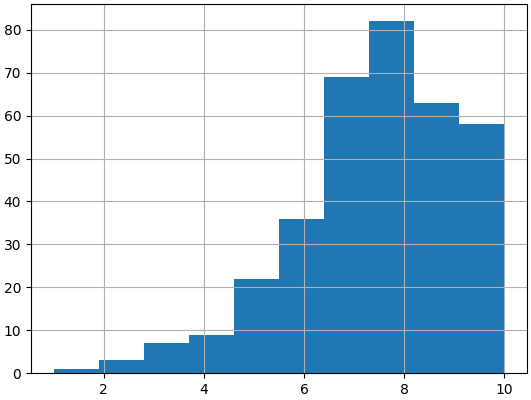
\includegraphics[width=0.7\textwidth]{./figures-and-tables/figure-1.png}};
        \node (n2) [above=0.25cm] at ($(n1)!0.5!(n1) - (7, 0)$) {\textbf{Count}};
        \node (n3) [above=0.25cm] at ($(n1)!0.5!(n1) - (0, 5.5)$) {\textbf{Favorability}};
    \end{tikzpicture}
    \label{fig:one}

    % \caption*{A figure}
    % \floatfoot{$^*$The outlying points at $X = {1,2,3}$ simply indicates there are one or more observations at these locations. It does not indicate t}
\end{figure}

The average response was 7.65 on a 10-point scale.
Excluding outliers, over 96 percent of responses fall into the normal range.
The average response in the normal range was about 7.81.
Table \ref{tab:desc_stats} summarizes statistics about favorability and the direct measure of coronavirus impact.
The table also includes summary results for the two causality questions.

% Table \ref{tab:desc_stats} describes summary statistics for the total sample and also distinctly describes three subsamples.
Table \ref{tab:desc_stats} reports statistics across the total population and also for three subpopulations.
The subpopulations include the normal range, the outlier population, and the Tens.
Because factors in Table \ref{tab:desc_stats} dummy variables,
with an exception for favorability,
the mean values for each variable can be interpreted as the proportion of the population
that affirms the response.

The Tens are those individuals that responded with a favorability of 10 to alternative credentials.
The Tens are not an outlier group, but inspection of this group assists in understanding the response distribution.
The Tens report a large perceived impact at a disproportionately high rate.
In contrast, no member of the negative outlier group also reports a large perceived impact of coronavirus.
% Group differences like this demonstrate that general results for the whole American population are to be taken lightly,
% and 
% The difference in perceived impact by group is important when conclusions about the American population are drawn from the discussion on coronavirus impact.

This data is consistent with external reporting that COVID-19 impacts most Americans\cite{demographic2020},
but it adds the wrinkle that most Americans consider the impact to be minor.
Perceived COVID-19 impact is another case where outliers and Tens importantly differ from the average.
The Tens report higher coronavirus impact while the outliers cluster around a medium impact response.

\begin{table}
    \caption{Summary Statistics for Factors of Interest}
    \resizebox{\columnwidth}{!}{
        {
\def\sym#1{\ifmmode^{#1}\else\(^{#1}\)\fi}
\begin{tabular}{llcc}
    \toprule
                              &                                   & \textbf{Average Hirability} & \textbf{Average Prestige} \\
    \midrule
    \textbf{Actual Schools}   &                                   &                             & 6.50                      \\
                              & \textbf{Accredited}               &                             & 7.05                      \\
                              & \textbf{Unaccredited}             &                             & 6.07                      \\
                              & \textbf{Difference}               &                             & 0.98                      \\
    \cmidrule{2-4}
                              & \textbf{Stipulated High Prestige} &                             & 6.72                      \\
                              & \textbf{Stipulated Low Prestige}  &                             & 6.23                      \\
                              & \textbf{Difference}               &                             & 0.49                      \\
    \cmidrule{2-4}
    \textbf{Vignette Schools} &                                   & 6.49                        & 6.21                      \\
                              & \textbf{Accredited}               & 6.97                        & 6.49                      \\
                              & \textbf{Unaccredited}             & 6.02                        & 5.93                      \\
                              & \textbf{Difference}               & 0.95                        & 0.56                      \\
    \cmidrule{2-4}
                              & \textbf{Stipulated High Prestige} & 7.59                        & 7.69                      \\
                              & \textbf{Stipulated Low Prestige}  & 5.63                        & 4.94                      \\
                              & \textbf{Difference}               & 1.96                        & 2.75                      \\
    %   \midrule
    % \textbf{Pooled}           &                                   &                             & 6.37                      \\
    %                           & \textbf{Accredited}               &                             & 6.77                      \\
    %                           & \textbf{Unaccredited}             &                             & 6.01                      \\
    %                           & \textbf{Difference}               &                             & 0.76                      \\
    %                           & \textbf{Stipulated High Prestige} &                             & 7.00                      \\
    %                           & \textbf{Stipulated Low Prestige}  &                             & 5.80                      \\
    %                           & \textbf{Difference}               &                             & 1.20                      \\
    \bottomrule
    \bottomrule
\end{tabular}
}

    }
    \label{tab:desc_stats}
\end{table}

Table \ref{tab:multiple_regs} provides factor coefficients for four interesting OLS models.
Model 1 is the adjusted R-squared maximizing model.
Model 4 is composed only of significant factors.
Model 2 is Model 4 plus a dummy for a large coronavirus impact.
Model 3 follows the same specification as Model 2, but Model 3 excludes outliers.

\begin{table}
    \caption{Table of Multiple Regressions with Favorability as Dependent Variable}
    \resizebox{\columnwidth}{!}{
        {
\def\sym#1{\ifmmode^{#1}\else\(^{#1}\)\fi}
\begin{tabular}{lcccccc}
\toprule
                                                   & \textbf{coef} & \textbf{std err} & \textbf{t} & \textbf{P$> |$t$|$} & \textbf{[0.025} & \textbf{0.975]}  \\
\midrule
\textbf{Intercept}                                 &       3.4814  &        0.431     &     8.071  &         0.000        &        2.633    &        4.330     \\
\textbf{conventional\_alt\_creds}                  &       0.4485  &        0.045     &     9.918  &         0.000        &        0.360    &        0.537     \\
\textbf{favor\_online\_ed}$^2$                     &       0.0993  &        0.035     &     2.843  &         0.005        &        0.031    &        0.168     \\
\textbf{covid\_ind\_remote\_large\_degree}         &       0.5613  &        0.206     &     2.721  &         0.007        &        0.156    &        0.967     \\
\textbf{covid\_ind\_fav\_online\_large\_degree}    &      -0.8037  &        0.309     &    -2.602  &         0.010        &       -1.411    &       -0.196     \\
\textbf{covid\_ind\_fav\_online\_moderate\_degree} &      -0.6581  &        0.243     &    -2.711  &         0.007        &       -1.136    &       -0.181     \\
\textbf{covid\_ind\_fav\_online\_slight\_degree}   &      -0.5347  &        0.251     &    -2.127  &         0.034        &       -1.029    &       -0.040     \\
\textbf{industry\_health}                          &       0.5461  &        0.288     &     1.894  &         0.059        &       -0.021    &        1.113     \\
\textbf{industry\_information\_technology}         &       0.3394  &        0.192     &     1.766  &         0.078        &       -0.039    &        0.717     \\
\textbf{industry\_manufacturing}                   &       0.6792  &        0.294     &     2.307  &         0.022        &        0.100    &        1.258     \\
\textbf{industry\_real\_estate}                    &       1.1427  &        0.645     &     1.770  &         0.078        &       -0.127    &        2.412     \\
\textbf{ethnicity\_hispanic}                       &       0.7559  &        0.414     &     1.827  &         0.069        &       -0.058    &        1.570     \\
\textbf{ethnicity\_other}                          &       1.5186  &        0.781     &     1.945  &         0.053        &       -0.017    &        3.054     \\
\textbf{ethnicity\_white\_caucasian}               &       0.4370  &        0.180     &     2.432  &         0.016        &        0.083    &        0.791     \\
\textbf{state\_georgia}                            &       1.2169  &        0.509     &     2.392  &         0.017        &        0.216    &        2.218     \\
\textbf{state\_iowa}                               &      -2.6606  &        0.882     &    -3.018  &         0.003        &       -4.395    &       -0.926     \\
\textbf{state\_kentucky}                           &      -1.2358  &        0.682     &    -1.812  &         0.071        &       -2.577    &        0.106     \\
\textbf{state\_ohio}                               &      -1.3443  &        0.638     &    -2.108  &         0.036        &       -2.599    &       -0.090     \\
\textbf{state\_pennsylvania}                       &      -0.9913  &        0.468     &    -2.116  &         0.035        &       -1.913    &       -0.070     \\
\bottomrule
\end{tabular}
% \end{center}
% \begin{center}
% \begin{tabular}{lclc}
% \toprule
% \textbf{Omnibus:}       & 23.897 & \textbf{  Durbin-Watson:     } &    2.218  \\
% \textbf{Prob(Omnibus):} &  0.000 & \textbf{  Jarque-Bera (JB):  } &   29.746  \\
% \textbf{Skew:}          & -0.558 & \textbf{  Prob(JB):          } & 3.47e-07  \\
% \textbf{Kurtosis:}      &  3.892 & \textbf{  Cond. No.          } &     124.  \\
% \bottomrule
% \end{tabular}
}

    }
    \label{tab:multiple_regs}
\end{table}

The direct effect of coronavirus appears to be positive and also insignificant.
The response indicating that a person has perceived a large impact from coronavirus is the only dummy
within this categorical variable to appear in any of these models of interest.
Notice that the large impact factor is invariant to the outlier subpopulation
because no negative outlier reported a large impact.

In a simple regression of the large coronavirus impact dummy on favorability,
the variable becomes more significant and important ($\beta = 0.46, p < 0.15$).
The two questions on causality\footnote{These include questions thirteen and fourteen in Appendix C.}
partial out the explanation from the direct measure.
This is evidence that a coronavirus-induced remote activity exposure accounts for most of the effect attributable to coronavirus.
% This should not be taken as evidence that coronavirus as a historical event has insignificant bearing on favorability.

The two causality questions are significant across models.
The coefficients range from half a point to a point, which indicates moderate importance.
The first causality question asks whether coronavirus caused an increased degree of remote activity for the respondent.
The coefficient on the dummy variable indicating a large coronavirus-induced increase to remote activity is positive.
This is consistent with the hypothesis of a positive exposure effect.

The second question on causality asks whether coronavirus-induced remote activities cause an increase
to favorability about remote learning.
The exact wording is:
``To what degree has coronavirus-induced remote activity improved your favorability to remote learning
(either for yourself or for other people)?''
Referring back to Table \ref{tab:desc_stats},
about 83.1 percent of the full population of Americans indicate a small,
medium, or large increase in favorability of remote learning
caused by coronavirus-induced remote activity.
% Other than "none", any response to this question constitutes evidence that coronavirus causes increased favorability to remote learning.
This study separately demonstrates a positive relationship between favorability to remote learning
and favorability to alternative credentials.
Taken together,
these two factors provide positive evidence toward the hypothesis that coronavirus-induced exposure to remote learning
results in an increase in favorability to alternative credentials.

The observation of nonzero responses to the factor for coronavirus-induced remote learning favorability is causal evidence.
The fact that these nonzero responses are negatively related to favorability is a non-causal association.
This association indicates that those who gained the most favorability also ended with less than average favorability,
while those with prior high favorability did not move much higher.
This interpretation is reinforced by referring back to the summary statistics in Table \ref{tab:desc_stats}.
Notice that the negative outlier group has the highest affirmative response for both a
medium increase in remote favorability
and also to a large increase in remote favorability.
On the other hand, the normal range has the highest response rate for a small increase to remote favorability.
A relatively small improvement for most respondents makes sense,
given that the median response is already near the maximum response.

Coronavirus-induced favorability to online education is distinct from a plain measure of favorability to online education.
The latter is labeled Favor Online Education within Table \ref{tab:multiple_regs},
and it is one of the two unique controls discussed in the Methodology.
This factor was most significant when modeled as a quadratic term.
A quadratic term captures marginal effects.
The coefficient for this term is positive, indicating a positive marginal effect.
Favorability to online education
and coronavirus-induced favorability to online education are moderately correlated (Pearson's $r=0.303$).
This demonstrates internal consistency among responses,
and it also adds weight to the explanation from exposure.

The other unique control is expected conventionality.
This factor is also significant, robust to specification, and important.
Expected conventionality and favorability to online education correlate moderately (Pearson's $r=0.445$).
Expected conventionality is uncorrelated to coronavirus-induced favorability to online education.
Respondents do not form an expectation that alternative credentials will be conventional in the future
after being exposed to coronavirus-induced remote activities.

Table \ref{tab:table_robust_reg} is a table of factors for a robust linear model (RLM).
Robust regression is useful in addressing samples in which outliers exist, so the robust model includes the whole sample.
Because RLM treats factors linearly, the coefficients are comparable to OLS coefficients.
This makes the model in Table \ref{tab:table_robust_reg} useful for factor analysis as well.
Specifically, the model in this table is a simple respecification of Model 4 from Table \ref{tab:multiple_regs} into RLM.
The main result in this table is that none of the effects of interest are importantly different between RLM and OLS specification.

\begin{table}
    \caption{Table of Robust Linear Model with Favorability as Dependent Variable}
    \resizebox{\columnwidth}{!}{
        {
\def\sym#1{\ifmmode^{#1}\else\(^{#1}\)\fi}
\begin{tabular}{lcccccc}
    \toprule
                                                    & \textbf{coef} & \textbf{std err} & \textbf{z} & \textbf{P$> |$z$|$} & \textbf{[0.025} & \textbf{0.975]} \\
    \midrule
    \textbf{Favor Online Education$^2$}             & 0.1083        & 0.033            & 3.289      & 0.001               & 0.044           & 0.173           \\
    \textbf{Expected Conventionality}               & 0.4566        & 0.042            & 10.855     & 0.000               & 0.374           & 0.539           \\
    \textbf{Large Change to Remote Activity}        & 0.6981        & 0.192            & 3.637      & 0.000               & 0.322           & 1.074           \\
    \textbf{Small Increase to Remote Favorability}  & -0.6117       & 0.236            & -2.595     & 0.009               & -1.074          & -0.150          \\
    \textbf{Medium Increase to Remote Favorability} & -0.7676       & 0.228            & -3.362     & 0.001               & -1.215          & -0.320          \\
    \textbf{Large Increase to Remote Favorability}  & -0.8345       & 0.290            & -2.874     & 0.004               & -1.404          & -0.265          \\
    \textbf{Industry, Health}                       & 0.5969        & 0.271            & 2.205      & 0.027               & 0.066           & 1.128           \\
    \textbf{Industry, Information Technology}       & 0.4016        & 0.180            & 2.237      & 0.025               & 0.050           & 0.754           \\
    \textbf{Industry, Manufacturing}                & 0.7399        & 0.277            & 2.672      & 0.008               & 0.197           & 1.282           \\
    \textbf{Ethnicity, Caucasian}                   & 0.3168        & 0.161            & 1.963      & 0.050               & 0.001           & 0.633           \\
    \textbf{Ethnicity, Other}                       & 1.7074        & 0.724            & 2.359      & 0.018               & 0.289           & 3.126           \\
    \textbf{State, Georgia}                         & 1.0604        & 0.479            & 2.212      & 0.027               & 0.121           & 2.000           \\
    \textbf{State, Ohio}                            & -1.0150       & 0.601            & -1.690     & 0.091               & -2.192          & 0.162           \\
    \textbf{State, Pennsylvania}                    & -0.8238       & 0.441            & -1.867     & 0.062               & -1.688          & 0.041           \\
    \textbf{Intercept}                              & 3.5185        & 0.401            & 8.785      & 0.000               & 2.734           & 4.303           \\
    \midrule
    \textbf{N}                                      & 350           &                  &            &                     &                 &                 \\
    \bottomrule
\end{tabular}
}

    }
    \label{tab:table_robust_reg}
\end{table}

The other control variables also exhibit some interesting effects.
Caucasians disproportionately attend and graduate from college,
leading some scholars to argue that higher education is an instrument of white supremacy\cite{hikido2016whitened, dennis2001skillful}.
Other scholars note that alternative learning providers support a higher rate of minority graduation.
As a result, support for alternative credentials is considered a workforce diversity strategy\cite{brown2017complex, jones2018alternative, rossiter2019designing}.
Given such prior research,
it is intuitive to expect a negative association between caucasian ethnicity and support for alternative credentials.
Opposite expectation, caucasian ethnic identification presents a significant positive coefficient in this study.

Information technology is a well-known stronghold of support for alternative education, including coding bootcamps.
Key skills in information technology are easily digitized and taught over the web.
This industry demands flexible instruction because it is associated with a uniquely high rate of technical obsolescence.
It is not surprising that it is positively associated with favorability.
It is surprising that it comes in third place among four industries with positive and significant favorability.

Health is an industry that has been historically difficult to digitize.
Shimizu et al. describe improvements to remote medical education from 2003 to 2013\cite{shimizu2014ten}.
They show, for example, that improvements to video quality over time were an important technological driver
of success for instruction on surgical techniques.
The historical difficulty of remote medical education and service delivery seems at tension with the present study.
The present study shows an important positive effect of the health industry on favorability.

The tension is resolved by a recognition of the recent flourishing of remote health technology.
Health education was enhanced, for example, through the application of virtual reality to simulation-based learning.
The Oculus Rift is a hardware device that improved virtual reality simulation quality after the year 2010\cite{giuseppe2015new}.
Three meta-analyses from the Digital Health Education Collaboration in 2019 confirm that modern virtual reality,
mobile digital education, and
digital problem-based learning methods are as effective or more effective than traditional learning methods\cite{kyaw2019virtual, dunleavy2019mobile, car2019digital}.

There are various political and cultural reasons for which favorability might vary by state, but the current analysis does not provide strong evidence toward any particular explanation.
Employment status was largely insignificant, but Model 1 hints at a weak positive effect among hiring managers.
Other controls are notably insignificant.
Gender, age, and level of education had no bearing on favorability.
The insignificance of age and education level provides weak evidence
against the hypotheses that older individuals or individuals who do have traditional degrees
have a disproportionate opposition to alternative credentials.

\section{Conclusions}

Results indicate that coronavirus as a historical event has significantly improved American favorability to alternative credentials.
The effect is not well-explained by the direct impact of coronavirus on an individual.
The effect is well-explained as a positive exposure effect that results from coronavirus-induced remote activities.
The largest gains in favorability accrue to individuals that began and ended with less than average favorability.

The introduction provided three explanations for improved favorability,
but this study most directly examined an explanation from exposure.
If the exposure effect had been weak and favorability improved anyway,
the other hypotheses would have become more important.
Given the effectiveness of the exposure-based explanation, the other two explanations are not considered independently important.
Arguments from organizational agility and normal strangeness may remain endogenously important.
For example, exposure to certain services might improve consumer favorability precisely because
organizational agility has enabled the development of quality products.

As is a cross-sectional analysis,
this study provides little ability to make confident forecasts about whether the favorability increase is transient or permanent.
With that caveat, there are three reasons to expect average favorability to remain near a score of eight out of ten.
The first reason is that this was the average score found in the analysis.
Barring contrary evidence, this point-estimate remains preferred.

The second reason is that there are reasons to expect favorability to increase and to decrease.
Without evidence on a significant difference in the magnitudes of effects in either direction,
a net expectation of stability results.
Mean regression is a reason to expect a favorability decrease.
Continuity of trend is a reason to expect an increase.

The third and strongest reason to expect favorability to remain near the present level is that
society has shifted and developed new norms in response to the pandemic.
Once society establishes new norms, there are numerous ways in which those norms reinforce themselves.
Status-quo bias and anchoring bias are relevant psychological forces.
Economic effects include the endowment effect and ordinary switching costs.
For example, an endowment effect might apply to a worker who is now remote and prefers not to return to a physical office.

This study indicates that the population supports alternative credentials.
Policy recommendations that facilitate this preference include improvements to federal recognition and social access.
Much of this work is already underway.
Many colleges now award credit for professional experience or nontraditional education.
Institutions like the American Council on Education (ACE)
have facilitated this effort through programs like the current ACE Apprenticeship Pathways project
and the now-defunct Alternative Credit Project (ACP)\cite{education_2021}.
Renewal of the ACP is an example of a public-private partnership that is feasible and would improve recognition of alternative credentials.

In 2012, The Heritage Foundation called for certain radical policy changes that would level the playing field between traditional and alternative educators.
While they did not go as far as to suggest eliminating accreditation,
they did advocate for removing accreditation agencies.
Heritage suggested the government should directly accredit courses rather than organizations\cite{burke2012accreditation}.
They also called for a decoupling of accreditation and federal funding.

Congress has yet to take Heritage up on the idea,
but rule changes from the Department of Education that took effect in July of 2020
have made accreditation easier\cite{weissman_2019}.
Further accreditation reform can incentivize competition in the university space,
essentially causing universities to compete with alternative providers on price and quality to a greater extent.
This would not drive support for alternative credentials directly,
but improving competition and removing barriers to entry in higher education seems beneficial for the market as a whole.

Removal of federal subsidies for higher education would reduce college prices and combat student debt,
but this is another unpopular reform.
A second-best solution would be to open the subsidy to alternative providers.
Section 127 of the Internal Revenue Code allows for employer educational assistance.
Previously, such assistance consisted of paying for new accredited education.
The CARES Act expanded Section 127 employer assistance
to include paying down student loans that currently exist from accredited prior education\cite{miller_2021}.
One small move that would improve access to alternative education
would be to modify the definition of educational assistance to include unaccredited learning.

In addition to public policy changes, industry and firm policy changes can facilitate the adoption of alternative credentials.
Several high-value corporations have dropped the requirement of a college degree\cite{team_2020}.
Other companies allow particular unaccredited credentials to fulfill a college degree requirement.
Alternative education providers have also begun providing a payment option using an income sharing agreement (ISA) rather than loans.
The income sharing agreement improves access by eliminating the need for student payment
until a student obtains employment involving a designated minimum salary.


% %%
% %%  bibliography
% %%

% \Urlmuskip=0mu plus 1mu\relax
\bibliographystyle{elsarticle-num}
\bibliography{./BibFile}

%%
%% curriculum vitae
%%
%% Note: brief CV based on Josh Ingber's CV and Jon Schuler's totally absent CV page
%% Josh Ref: https://search-proquest-com.mutex.gmu.edu/pqdtlocal1006610/docview/2428073176/55635F0359FC4ECCPQ/1?accountid=14541
%% Jon Ref: https://search-proquest-com.mutex.gmu.edu/pqdtlocal1006610/docview/305048351/C349E532582D467APQ/1?accountid=14541

\cvpage

\noindent John Vandivier received his Ph.D. in Economics from George Mason University (GMU) in 2021.
John specialized in the fields of Austrian Economics and Public Choice Economics during his doctoral studies.
His dissertation includes a focus on applied microeconomic analysis, education economics, statistical analysis, and light experimental analysis.
In 2015, John earned a Master of Public Policy (MPP) with an emphasis in Fiscal Policy from George Mason University.
John received a Bachelor of Science (BS) with a double major in Economics in Political Science from the University of Houston in 2012.
John is currently employed as a Principal Software Developer affiliated with Blue Cross Blue Shield of North Carolina.

\end{document}
